%!TEX root = main.tex


\section{String Diagrams}\label{ssec:mken_diagrams}


We use a string diagram notation to represent probabilistic functions. This is a notation created for reasoning about abstract Markov categories, and is somewhat different to existing graphical languages. The main difference is that in our notation wires represent variables and boxes (which are like nodes in directed acyclic graphs) represent probabilistic functions. Standard directed acyclic graphs annotate nodes with variable names and represent probabilistic functions implicitly. The advantage of explicitly representing probabilistic functions is that we can write equations involving graphics. This is introduced in Section \ref{ssec:mken_diagrams}.

We make use of string diagram notation for probabilistic reasoning. Graphical models are often employed in causal reasoning, and string diagrams are a kind of graphical notation for representing Markov kernels. The notation comes from the study of Markov categories, which are abstract categories that represent models of the flow of information. For our purposes, we don't use abstract Markov categories but instead focus on the concrete category of Markov kernels on standard measurable sets.

A coherence theorem exists for string diagrams and Markov categories. Applying planar deformation or any of the commutative comonoid axioms to a string diagram yields an equivalent string diagram. The coherence theorem establishes that any proof constructed using string diagrams in this manner corresponds to a proof in any Markov category \citep{selinger_survey_2011}. More comprehensive introductions to Markov categories can be found in \citet{fritz_synthetic_2020,cho_disintegration_2019}.

\subsection{Elements of string diagrams}\label{sec:string_diagram_elements}

In the string, Markov kernels are drawn as boxes with input and output wires, and probability measures (which are Markov kernels with the domain $\{*\}$) are represented by triangles:

\begin{align}
\kernel{K}&:=\begin{tikzpicture}[baseline={([yshift=-.5ex]current bounding box.center)}]
    \path (0,0) node (A) {}
    ++ (0.5,0) node[kernel] (K) {$\kernel{K}$}
    ++ (0.5,0) node (B) {};
    \draw (A) -- (K) -- (B);
\end{tikzpicture}\\
\mu&:= \begin{tikzpicture}[baseline={([yshift=-.5ex]current bounding box.center)}]
    \path (0,0) node[dist] (K) {$\kernel{P}$}
    ++ (0.5,0) node (B) {};
    \draw (K) -- (B);
\end{tikzpicture}
\end{align}

Given two Markov kernels $\kernel{L}:X\kto Y$ and $\kernel{M}:Y\kto Z$, the product $\kernel{L}\kernel{M}$ is represented by drawing them side by side and joining their wires:

\begin{align}
    \kernel{L}\kernel{M}:= \begin{tikzpicture}[baseline={([yshift=-.5ex]current bounding box.center)}]
    \path (0,0) node (A) {$X$}
    ++ (0.5,0) node[kernel] (K) {$\kernel{K}$}
    ++ (0.7,0) node[kernel] (M) {$\kernel{M}$}
    ++ (0.5,0) node (B) {$Z$};
    \draw (A) -- (K) -- (M) -- (B);
\end{tikzpicture}
\end{align}

Given kernels $\kernel{K}:W\kto Y$ and $\kernel{L}:X\kto Z$, the tensor product $\kernel{K}\otimes\kernel{L}:W\times X\kto Y\times Z$ is graphically represented by drawing kernels in parallel:

\begin{align}
    \kernel{K}\otimes \kernel{L}&:=\begin{tikzpicture}[baseline={([yshift=-.5ex]current bounding box.center)}]
    \path (0,0) node (A) {$W$}
    ++ (0.5,0) node[kernel] (K) {$\kernel{K}$}
    ++ (0.5,0) node (B) {$Y$};
    \path (0,-0.5) node (C) {$X$}
    ++ (0.5,0) node[kernel] (L) {$\kernel{L}$}
    ++ (0.5,0) node (D) {$Z$};
    \draw (A) -- (K) -- (B);
    \draw (C) -- (L) -- (D);
\end{tikzpicture}
\end{align}

Given $\prob{K}:X\kto Y$ and $\prob{L}:Y\times X\kto Z$, the semidirect product is graphically represented by connecting $\kernel{K}$ and $\kernel{L}$ and keeping an extra copy

\begin{align}
    \prob{K}\cprod\prob{L}:&= \text{Copy}_X(\prob{K}\otimes \text{id}_X)(\text{Copy}_Y\otimes\text{id}_X )(\text{id}_Y \otimes \prob{L})\\
                            &= \tikzfig{copy_product}
\end{align}

A space $X$ is identified with the identity kernel $\mathrm{id}^X:X\to \Delta(\sigalg{X})$. A bare wire represents the identity kernel:

\begin{align}
\mathrm{Id}^X:=\begin{tikzpicture}
\path (0,0) node (X) {$X$}
++(2,0) node (Y) {$X$};
\draw (X) -- (Y);
\end{tikzpicture}
\end{align}

Product spaces $X\times Y$ are identified with tensor product of identity kernels $\mathrm{id}^X\otimes \mathrm{id}^Y$. These can be represented either by two parallel wires or by a single wire representing the identity on the product space $X\times Y$:
\begin{align}
X\times Y \cong \mathrm{Id}^X\otimes \mathrm{Id}^Y &:= 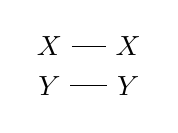
\begin{tikzpicture}
\path (0,0) node (E) {$X$}
++(1,0) node (F) {$X$}
(0,-0.5) node (F1) {$Y$}
+(1,0) node (G) {$Y$};
\draw (E) -- (F);
\draw (F1) -- (G);
\end{tikzpicture}\\
&= 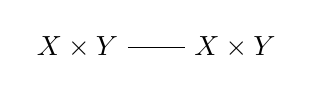
\begin{tikzpicture}
\path (0,0) node (X) {$X\times Y$}
++(2,0) node (Y) {$X\times Y$};
\draw (X) -- (Y);
\end{tikzpicture}
\end{align}

A kernel $\kernel{L}:X\to \Delta(\mathcal{Y}\otimes\mathcal{Z})$ can be written using either two parallel output wires or a single output wire, appropriately labeled:

\begin{align}
&\begin{tikzpicture}
\path (0,0) node (E) {$X$}
++ (1,0) node[kernel] (L) {$\kernel{L}$}
++ (1,0.15) node (F) {$Y$}
+(0,-0.3) node (G) {$Z$};
\draw (E) -- (L);
\draw ($(L.east) + (0,0.15)$) -- (F);
\draw ($(L.east)+ (0,-0.15)$) -- (G);
\end{tikzpicture}\\
&\equiv\\
&\begin{tikzpicture}
\path (0,0) node (E) {$X$}
++ (1,0) node[kernel] (L) {$\kernel{L}$}
++ (1.5,0) node (F) {$Y\times Z$};
\draw (E) -- (L) -- (F);
\end{tikzpicture}
\end{align}

We read diagrams from left to right (this is somewhat different to \citet{fritz_synthetic_2020,cho_disintegration_2019,fong_causal_2013} but in line with \citet{selinger_survey_2011}), and any diagram describes a set of nested products and tensor products of Markov kernels. There are a collection of special Markov kernels for which we can replace the generic ``box'' of a Markov kernel with a diagrammatic elements that are visually suggestive of what these kernels accomplish.

\subsection{Special maps}

\begin{definition}[Identity map]\label{def:ident_k}
The identity map $\text{Id}_X:X\kto X$ defined by $(\text{id}_X)(A|x)= \delta_x(A)$ for all $x\in X$, $A\in\sigalg{X}$, is represented by a bare line.
\begin{align}
    \mathrm{id}_X&:=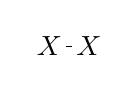
\begin{tikzpicture}[baseline={([yshift=-.5ex]current bounding box.center)}]
    \path (0,0) node (A) {$X$} ++ (0.5,0) node (B) {$X$};
    \draw (A) -- (B);
\end{tikzpicture}
\end{align}
\end{definition}

\begin{definition}[Erase map]\label{def:erase}
Given some 1-element set $\{*\}$, the erase map $\text{Del}_X:X\kto \{*\}$ is defined by $(\text{Del}_X)(*|x) = 1$ for all $x\in X$. It ``discards the input''. It looks like a lit fuse:
\begin{align}
    \text{Del}_X&:=\begin{tikzpicture}[baseline={([yshift=-.5ex]current bounding box.center)}]
    \path (0,0) ++ (1,0) node (B) {$X$};
    \draw[-{Rays[n=8]}] (A) -- (B);
\end{tikzpicture}
\end{align}
\end{definition}

\begin{definition}[Swap map]\label{def:swap}
The swap map $\text{Swap}_{X,Y}:X\times Y\kto Y\times X$ is defined by $(\text{Swap}_{X,Y})(A\times B|x,y)=\delta_x(B)\delta_y(A)$ for $(x,y)\in X\times Y$, $A\in \sigalg{X}$ and $B\in \sigalg{Y}$. It swaps two inputs and is represented by crossing wires:
\begin{align}
    \text{Swap}_{X,Y} &:=  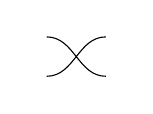
\begin{tikzpicture}[baseline={([yshift=-.5ex]current bounding box.center)}]
        \path (0,0) node (A) {} 
        + (0,-0.5) node (B) {}
        ++ (1,0) node (C) {}
        + (0,-0.5) node (D) {};
        \draw (A) to [out=0,in=180] (D) (B) to [out=0, in=180] (C);
    \end{tikzpicture}
\end{align}
\end{definition}

\begin{definition}[Copy map]\label{def:copy}
The copy map $\text{Copy}_X:X\kto X\times X$ is defined by $(\text{Copy}_X)(A\times B|x)=\delta_x(A)\delta_x(B)$ for all $x\in X$, $A,B\in \sigalg{X}$. It makes two identical copies of the input, and is drawn as a fork:
\begin{align}
    \text{Copy}_X&:=\begin{tikzpicture}[baseline={([yshift=-.5ex]current bounding box.center)}]
    \path (0,0) node (A) {$X$} 
    ++ (0.5,0) node[copymap] (copy0) {}
    ++ (0.5,0.15) node (B) {$X$}
    + (0,-0.3) node (C) {$X$};
    \draw (A) -- (copy0) to [out=45,in=180] (B) (copy0) to [out=-45, in=180] (C);
\end{tikzpicture}
\end{align}
\end{definition}

\begin{definition}[$n$-fold copy map]
The $n$-fold copy map $\text{Copy}^n_X:X\kto X^n$ is given by the recursive definition
\begin{align}
    \text{Copy}^1_X &= \text{Copy}_X\\
    \text{Copy}^n_X &= \tikzfig{n_fold_copy} &n>1
\end{align}
\end{definition}

\paragraph{Plates}\label{pgph:plates}

In a string diagram, a plate that is annotated $i\in A$ means the tensor product of the $|A|$ elements that appear inside the plate. A wire crossing from outside a plate boundary to the inside of a plate indicates an $|A|$-fold copy map, which we indicate by placing a dot on the plate boundary. For our purposes, we do not define anything that allows wires to cross from the inside of a plate to the outside; wires must terminate within the plate.

Thus, given $\kernel{K}_i:X\kto Y$ for $i\in A$,

\begin{align}
    \bigotimes_{i\in A} \kernel{K}_i &:= \tikzfig{plate_without_copymap}
    \text{Copy}^{|A|}_X(\bigotimes_{i\in A} \kernel{K}_i) &:= \tikzfig{plate_with_copymap}
\end{align}

\subsection{Commutative comonoid axioms}

Diagrams in Markov categories satisfy the commutative comonoid axioms.

\begin{align}
    \tikzfig{ccom_lhs} = \tikzfig{ccom_rhs}\label{eq:ccom_1}
\end{align}
\begin{align}
    \tikzfig{ccom2_lhs} = \tikzfig{ccom2_mhs} = \tikzfig{ccom2_rhs}\label{eq:ccom2_del}
\end{align}
\begin{align}
    \tikzfig{ccom3_lhs} = \tikzfig{ccom3_rhs} \label{eq:ccom3_swap}
\end{align}
as well as compatibility with the monoidal structure
\begin{align}
    \tikzfig{mstruct1_lhs} &= \tikzfig{mstruct1_rhs}\\
    \tikzfig{mstruct2_lhs} &= \tikzfig{mstruct2_rhs}
\end{align}
and the naturality of \emph{Del}, which means that
\begin{align}
    \tikzfig{naturality_lhs} &= \tikzfig{naturality_rhs}\label{eq:nat}
\end{align}


\subsection{Manipulating String Diagrams}\label{sssec:string_diagram_manipulation}

Planar deformations along with the applications of Equations \eqref{eq:ccom_1} through to Equation \eqref{eq:nat} are almost the only rules we have for transforming one string diagram into an equivalent one. One further rule is given by Theorem \ref{th:fong_det_kerns}.

\begin{theorem}[Copy map commutes for deterministic kernels \citep{fong_causal_2013}]\label{th:fong_det_kerns}
For $\kernel{K}:X\kto Y$
\begin{align}
	\tikzfig{deterministic_copymap_commute}
\end{align}
holds iff $\kernel{K}$ is deterministic.
\end{theorem}

\subsubsection{Examples}

String diagrams can always be converted into definitions involving integrals and tensor products. A number of shortcuts can help to make the translations efficiently.

For arbitrary $\kernel{K}:X\times Y\kto Z$, $\kernel{L}:W\kto Y$

\begin{align}
    \tikzfig{identity_tensor_L} &= (\text{id}_X\otimes \kernel{L})\kernel{K}\\
    [(\text{id}_X\otimes \kernel{L})\kernel{K}](A|x,w) &= \int_{Y}\int_X   \kernel{K}(A|x',y')\kernel{L}(\mathrm{d}y'|w)\delta_x(\mathrm{d}x')\\
                                           &= \int_Y  \kernel{K}(A|x,y') \kernel{L}(dy'|w)
\end{align}

That is, an identity map ``passes its input directly to the next kernel''. 

For arbitrary $\kernel{K}: X\times Y\times Y\kto Z$:

\begin{align}
 \tikzfig{identity_tensor_copy} &= (\text{id}_X\otimes \text{Copy}_Y)\kernel{K}\\
 [(\text{id}_X\otimes \text{Copy}_Y)\kernel{K}](A|x,y) &= \int_Y\int_Y \kernel{K}(A|x,y',y'') \delta_y(\mathrm{d}y')\delta_y(\mathrm{d}y'')\\
                                           &= \kernel{K}(A|x,y,y)
\end{align}

That is, the copy map ``passes along two copies of its input'' to the next kernel in the product. 

For arbitrary $\kernel{K}:X\times Y\kto Z$

\begin{align}
    \tikzfig{swap_example} &= \text{Swap}_{YX} \kernel{K}\\
    (\text{Swap}_{YX}\kernel{K})(A|y,x) &= \int_{X\times Y} \kernel{K}(A|x',y')\delta_y(\mathrm{d}y')\delta_x(\mathrm{d}x')\\
                                        &= \kernel{K}(A|x,y)
\end{align}

The swap map before a kernel switches the input arguments.

For arbitrary $\kernel{K}:X\kto Y\times Z$

\begin{align}
    \tikzfig{swap_example_2} &= \kernel{K}\text{Swap}_{YZ}\\
    (\kernel{K}\text{Swap}_{YZ})(A\times B|x) &= \int_{Y\times Z} \delta_{y}(B)\delta_{z}(A)\kernel{K}(\mathrm{d}y\times\mathrm{d}z|x)\\
    &= \int_{B\times A} \kernel{K}(\mathrm{d}y\times\mathrm{d}z|x)\\
    &= \kernel{K}(B\times A|x)
\end{align}

Given $\kernel{K}:X\kto Y$ and $\kernel{L}:Y\kto Z$:

\begin{align}
	(\kernel{K}\cprod \kernel{L})(\mathrm{id}_{Y}\otimes \mathrm{Del}_Z) &= \tikzfig{semidirect_K_L}\\
	 &= \tikzfig{semidirect_K_L_2} &\text{by Eq. \eqref{eq:nat}}\\
	 &= \tikzfig{semidirect_K_L_3} &\text{by Eq. \eqref{eq:ccom2_del}}
\end{align}

Thus the action of the $\text{Del}$ map is to marginalise over the deleted wire. With integrals, we can write

\begin{align}
	(\kernel{K}\cprod \kernel{L})(\mathrm{id}_{Y}\otimes \mathrm{Del}_Z)(A\times\{*\}|x) &= \int_{Y}\int_{\{*\}}\delta_y(A)\delta_{*}(\{*\})\kernel{L}(\mathrm{d}z|y)\kernel{K}(\mathrm{d}y|x)\\
	&= \int_A \kernel{K}(\mathrm{d}y|x)\\
	&= \kernel{K}(A|x)
\end{align}

\section{Symmetries of conditional probabilities}\label{app:io_contract_examples}

\subsection{Equality of equally sized contractions}\label{sec:equal_condits}

This is the proof of Theorem \ref{th:equal_of_condits}.

All swaps can be written as a product of transpositions, so proving that a property holds for all finite transpositions is enough to show it holds for all finite swaps. It's useful to define a notation for transpositions.

\begin{definition}[Finite transposition]
Given two equally sized sequences $A,B\in \mathbb{N}^n$ with $A=(a_i)_{i\in [n]}$, $B=(b_i)_{i\in [n]}$, ${A\rightarrow B}:\mathbb{N}\to \mathbb{N}$ is the permutation such that 
\begin{align}
    [A\rightarrow B](a_i) = b_i
\end{align}that sends the $i$th element of $A$ to the $i$th element of $B$ and vise versa. Note that $B\rightarrow A$ is the inverse of $A\rightarrow B$.
\end{definition}

Lemma \ref{lem:infinitely_extended_kernels} is used to extend conditional probabilities of finite sequences to infinite ones. 

\begin{lemma}[Infinitely extended kernels]\label{lem:infinitely_extended_kernels}
Given a collection of Markov kernels $\kernel{K}_i:W\times X^{\mathbb{N}}\kto Y^i$ for all $i\in \mathbb{N}$, if we have for every $j>i$
\begin{align}
    \kernel{K}_j(\text{id}_{Y^i}\otimes \text{Del}_{Y^{j-i}}) &= \kernel{K}_i\otimes \text{Del}_{X^{j-i}}\label{eqApp:marginalise_comb}
\end{align} 
then there is a unique Markov kernel $\kernel{K}:X^{\mathbb{N}}\kto Y^{\mathbb{N}}$ such that for all $i,j\in \mathbb{N}$,$j>i$
\begin{align}
    \kernel{K}(\text{id}_{Y^i}\otimes \text{Del}_{Y^{\mathbb{N}}})&= \kernel{K}_i\otimes \text{Del}_{X^{j-i}}
\end{align}
\end{lemma}

\begin{proof}
Take any $x\in X^{\mathbb{N}}$ and let $x_{|m}\in X^n$ be the first $n$ elements of $x$. By Equation \eqref{eqApp:marginalise_comb}, for any $A_i\in \sigalg{Y}$, $i\in [m]$
\begin{align}
    \kernel{K}_n(\bigtimes_{i\in [m]}A_i\times Y^{n-m}|x_{|n}) &= \kernel{K}_m(\bigtimes_{i\in [m]}A_i|x_{|m})
\end{align}

Furthermore, by the definition of the $\mathrm{Swap}$ map for any permutation $\rho:[n]\to[n]$
\begin{align}
    \kernel{K}_n\mathrm{Swap}_{\rho}(\bigtimes_{i\in [m]}A_{\rho(i)}\times Y^{n-m}|x_{|n}) &= \kernel{K}_n(\bigtimes_{i\in [m]}A_{i}\times Y^{n-m}|x_{|n})
\end{align}
thus by the Kolmogorov Extension Theorem \citep{cinlar_probability_2011}, for each $x\in X^{\mathbb{N}}$ there is a unique probability measure $\prob{Q}_x\in \Delta(Y^{\mathbb{N}}$ satisfying
\begin{align}
    \prob{Q}_x(\bigtimes_{i\in [n]}A_i\times Y^{\mathbb{N}}) &= \kernel{K}_n(\bigtimes_{i\in [n]}A_{\rho(i)}|x_{[n]})\label{eqApp:q_is_Markov}
\end{align}

Furthermore, for each $\{A_i\in\sigalg{Y}|i\in \mathbb{N}\}$, $n\in \mathbb{N}$ note that for $p>n$
\begin{align}
\prob{Q}_x(\bigtimes_{i\in[n]} A_i \times Y^{\mathbb{N}})&\geq \prob{Q}_x(\bigtimes_{i\in [p]} A_i\times Y^{\mathbb{N}})\\
&\geq \prob{Q}_x(\bigtimes_{i\in \mathbb{N}} A_i)
\end{align}
so by the Monotone convergence theorem, the sequence $\prob{Q}_x(\bigtimes_{i\in[n]} A_i)$ converges as $n\to \infty$ to $\prob{Q}_x(\bigtimes_{i\in\mathbb{N}} A_i)$. $x\mapsto \prob{Q}_x^{\RV{Z}_n}(\bigtimes_{i\in[n]} A_i)$ is measurable for all $n$, $\{A_i\in\sigalg{Y}|i\in \mathbb{N}\}$ by Equation \eqref{eqApp:q_is_Markov}, and so $x\mapsto Q_x$ is also measurable.

Thus $x\mapsto Q_x$ is the desired Markov kernel $\kernel{K}$.
\end{proof}

\begin{corollary}\label{cor:equal_subconditionals}
Given $(\prob{P}_C,\Omega,\sigalg{F})$, $\RV{W}:\Omega\to V$ and two pairs of sequences $(\RV{V},\RV{X}):=(\RV{V}_i,\RV{X}_i)_{i\in\mathbb{N}}$ and $(\RV{Y},\RV{Z}):=(\RV{Y}_i,\RV{Z}_i)_{i\in \mathbb{N}}$ with corresponding variables taking values in the same sets $V=Y$ and $X=Z$, if $(\prob{P}_C,\RV{V},\RV{X})$ and $(\prob{P}_C,\RV{Y},\RV{Z})$ are both local over $\RV{W}$ and
\begin{align}
    \prob{P}^{\RV{X}_{[n]}|\RV{W}\RV{V}_{[n]}} &= \prob{P}^{\RV{Z}_{[n]}|\RV{W}\RV{Y}_{[n]}}
\end{align}
for all $n\in\mathbb{N}$ then
\begin{align}
    \prob{P}^{\RV{X}|\RV{W}\RV{V}} &= \prob{P}^{\RV{Z}|\RV{W}\RV{Y}}
\end{align}
\end{corollary}

\begin{proof}
By assumption of locality
\begin{align}
    \prob{P}^{\RV{X}_{[n]}|\RV{W}\RV{V}_{[n]}}\otimes\mathrm{Del}_{W^\mathbb{N}} &= \prob{P}^{\RV{X}|\RV{W}\RV{V}}(\mathrm{id}_{X^n}\otimes \mathrm{Del}_{X^{\mathbb{N}}})\\
    \prob{P}^{\RV{Z}_{[n]}|\RV{W}\RV{Y}_{[n]}}\otimes\mathrm{Del}_{W^\mathbb{N}} &= \prob{P}^{\RV{Z}|\RV{W}\RV{Y}}(\mathrm{id}_{X^n}\otimes \mathrm{Del}_{X^{\mathbb{N}}})
\end{align}
hence for all $n,m>n$
\begin{align}
    \prob{P}^{\RV{X}_{[m]}|\RV{W}\RV{V}_{[m]}}(\mathrm{id}_{X^n}\otimes \mathrm{Del}_{X^{m-n}}) &= \prob{P}^{\RV{Z}_{[m]}|\RV{V}\RV{Y}_{[m]}}(\mathrm{id}_{X^n}\otimes \mathrm{Del}_{X^{m-n}})\\
    &= \prob{P}^{\RV{X}_{[n]}|\RV{W}\RV{V}_{[n]}}\otimes\mathrm{Del}_{W^{m-n}}
\end{align}
and, in particular, by lemma \ref{lem:infinitely_extended_kernels}, $\prob{P}^{\RV{X}|\RV{W}\RV{V}}$ and $\prob{P}^{\RV{Z}|\RV{W}\RV{Y}}$ are the limits of the same sequence.
\end{proof}

\begin{reptheorem}{th:equal_of_condits}
Given a sequential input-output model $(\prob{P}_C,\RV{D},\RV{Y})$ and some $\RV{W}$, $\prob{P}_\alpha^{\RV{Y}|\RV{WD}}$ is IO contractible over $\RV{W}$ if and only if for all subsequences $A,B\subset \mathbb{N}^{|A|}$ and for every $\alpha$
\begin{align}
    \prob{P}_\alpha^{\RV{Y}_A|\RV{WD}_{A,\mathbb{N}\setminus A}} &= \prob{P}_\alpha^{\RV{Y}_B|\RV{WD}_{B,\mathbb{N}\setminus B}}\\
    &= \prob{P}_\alpha^{\RV{Y}_A|\RV{WD}_A}\otimes \text{del}_{D^{|\mathbb{N}\setminus A|}}
\end{align}
\end{reptheorem}

\begin{proof}
Only if:
For $Z\in \mathbb{N}^{|A|}$, let $\text{del}_{Z^\complement}$ be the Markov kernel associated with the map that sends $\RV{Y}$ to $\RV{Y}_Z:=(\RV{Y}_i)_{i\in Z}$.

If $A$ is finite, then let $n:=|A|$ and by exchange commutativity
\begin{align}
        \prob{P}_\alpha^{\RV{Y}_A|\RV{WD_{A,\mathbb{N}\setminus A}}}&= \prob{P}_\alpha^{\RV{Y}_A|\RV{WD_{A\rightarrow [n]}}}\\
         &= \prob{P}_\alpha^{\RV{Y}|\RV{WD_{A\rightarrow [n]}}}\text{del}_{A^{\complement}}\\
        &=  \prob{P}_\alpha^{\RV{Y}_{[n]\rightarrow A}|\RV{WD}}\text{del}_{A^{\complement}}
\end{align}
Use the fact that $[n]\rightarrow A \circ B\rightarrow [n]= B\rightarrow A$ and apply exchange commutativity to get
\begin{align}
    \prob{P}_\alpha^{\RV{Y}_{[n]\rightarrow A}|\RV{WD}}\kernel{F}_{\Pi_{A}} &= \prob{P}_\alpha^{\RV{Y}_{B\rightarrow A}|\RV{WD}_{B\rightarrow [n]}}\text{del}_{A^{\complement}}\\
    &= \prob{P}_\alpha^{\RV{Y}|\RV{WD}_{B\rightarrow [n]}}\text{del}_{B^{\complement}}\\
    &= \prob{P}_\alpha^{\RV{Y}_B|\RV{WD_{B,\mathbb{N}\setminus B}}}
\end{align}

if $A$ is infinite, then we can take finite subsequences $A_m$ that are the first $m$ elements of $A$ and similarly for $B_m$. Then by previous reasoning
\begin{align}
            \prob{P}_\alpha^{\RV{Y}_{A_m}|\RV{WD_{A_m\rightarrow [m]}}} &= \prob{P}_\alpha^{\RV{Y}_{[m]}|\RV{WD}}\\
        &= \prob{P}_\alpha^{\RV{Y}_{B_m}|\RV{WD_{B_m\rightarrow [m]}}}
\end{align}
then by Corollary \ref{cor:equal_subconditionals}
\begin{align}
\prob{P}_\alpha^{\RV{Y}_A|\RV{WD_{A\rightarrow [n]}}}=\prob{P}_\alpha^{\RV{Y}_{B_m}|\RV{WD_{B_m\rightarrow [m]}}}
\end{align}

Finally, by locality
\begin{align}
    \prob{P}_\alpha^{\RV{Y}_A|\RV{WD_{A\rightarrow [n]}}} &= \prob{P}_\alpha^{\RV{Y}_A|\RV{WD}_A}\otimes \text{Del}_{D^{|\mathbb{N}\setminus A}}
\end{align}

If:
Taking $A=[n]$ for all $n$ establishes locality, and taking $A=(\rho(i))_{i\in \mathbb{N}}$ for arbitrary finite permutation $\rho$ establishes exchange commutativity.
\end{proof}

\subsection{Examples of symmetries}\label{app:examples_symmetries}

These are the examples referenced in Section \ref{sec:ccontracibility}. Example \ref{ex:no_implication} shows that neither locality nor exchange commutativity is implied by the other.

\begin{example}\label{ex:no_implication}
We prove the claim by way of presenting counterexamples.

First, a model that exhibits exchange commutativity but not locality. Suppose $D=Y=\{0,1\}$ and $\prob{P}_C^{\RV{Y}|\RV{D}}:D^{\mathbb{N}}\kto Y^{\mathbb{N}}$ is given by
\begin{align}
    \prob{P}_C^{\RV{Y}|\RV{D}}(\bigtimes_{i\in\mathbb{N}} A_i |(d_i)_{i\in\mathbb{N}}) &= \prod_{i\in \mathbb{N}} \delta_{\lim_{n\to\infty} \sum_{i\in\mathbb{N}} \frac{d_i}{n}}(A_i)
\end{align}
for some sequence $(d_i)_{i\in\mathbb{N}}$ such that this limit exists. Then for any finite permutation $\rho$
\begin{align}
    \prob{P}_C^{\RV{Y}_\rho|\RV{D}_\rho}(\bigtimes_{i\in\mathbb{N}} A_i |(d_i)_{i\in\mathbb{N}}) &= \prod_{i\in \mathbb{N}} \delta_{\lim_{n\to\infty} \sum_{i\in\mathbb{N}} \frac{d_{\rho^{-1}(i)}}{n}}(A_{\rho^{-1}(i)})\\
    &= \prob{P}_C^{\RV{Y}|\RV{D}}(\bigtimes_{i\in\mathbb{N}} A_i |(d_i)_{i\in\mathbb{N}})
\end{align}
so $(\prob{P}_C,\RV{D},\RV{Y})$ commutes with exchange, but
\begin{align}
    \prob{P}_C^{\RV{Y}_1|\RV{D}}(A_1 |0,1,1,1....) &= \delta_1(A_1)\\
    \prob{P}_C^{\RV{Y}_1|\RV{D}}(A_1 |0,0,0,0....) &= \delta_0(A_1)
\end{align}
so $(\prob{P}_C,\RV{D},\RV{Y})$ is not local.

Next, a model that satisfies locality but does not commute with exchange. Suppose again $D=Y=\{0,1\}$ and $\prob{P}_C^{\RV{Y}|\RV{D}}:D^{\mathbb{N}}\kto Y^{\mathbb{N}}$ is given by
\begin{align}
    \prob{P}_C^{\RV{Y}|\RV{D}}(\bigtimes_{i\in\mathbb{N}} A_i |(d_i)_{i\in\mathbb{N}}) &= \prod_{i\in \mathbb{N}} \delta_i(A_i)
\end{align}
then
\begin{align}
    \prob{P}_C^{\RV{Y}_\rho|\RV{D}_\rho}(\bigtimes_{i\in\mathbb{N}} A_i |(d_i)_{i\in\mathbb{N}}) &= \prod_{i\in \mathbb{N}} \delta_i(A_{\rho^{-1}(i)})\\
    &\neq \prod_{i\in \mathbb{N}} \delta_i(A_{i})\\
    =\prob{P}_C^{\RV{Y}|\RV{D}}(\bigtimes_{i\in\mathbb{N}} A_i |(d_i)_{i\in\mathbb{N}})
\end{align}
so $(\prob{P}_C,\RV{D},\RV{Y})$ does not commute with exchange but for all $n$
\begin{align}
    \prob{P}_C^{\RV{Y}_{[n]}|\RV{D}}(\bigtimes_{i\in[n]} A_i |(d_i)_{i\in\mathbb{N}}) &= \prod_{i\in [n]} \delta_i(A_{\rho^{-1}(i)})\\
    &= \prob{P}_C^{\RV{Y}_{[n]}|\RV{D}}(\bigtimes_{i\in[n]} A_i |(0)_{i\in\mathbb{N}})
\end{align}
so $(\prob{P}_C,\RV{D},\RV{Y})$ is local.
\end{example}

Although locality seems to an assumption that there is no interference between inputs and outputs of different indices, by itself it actually permits models with certain kinds of interference. This is shown in Example \ref{ex:interference_w_locality}.

\begin{example}\label{ex:interference_w_locality}
Consider an experiment where I first flip a coin and record the results of this flip as the outcome $\RV{Y}_1$ of ``step 1''. Subsequently, I can either copy the outcome from step 1 to the result for ``step 2'' (this is the input $\RV{D}_1=0$), or flip a second coin use this as the input for step 2 (this is the input $\RV{D}_1=1$). $\RV{D}_2$ is an arbitrary single-valued variable. Then for all $d_1, d_2$
\begin{align}
    \prob{P}^{\RV{Y}_1|\RV{D}}(y_1|d_1,d_2) &= 0.5\\
    \prob{P}^{\RV{Y}_2|\RV{D}}(y_2|d_1,d_2) &= 0.5
\end{align}
Thus the marginal distribution of both experiments in isolation is $\text{Bernoulli}(0.5)$ no matter what choices I make, but the input $\RV{D}_1$ affects the joint distribution of the results of both steps, which is not ruled out by locality.
\end{example}

\subsection[Representation]{Representation theorem preliminaries}\label{app:representation_proof}

This is the proof of Lemmas \ref{th:table_rep_kernel} and \ref{lem:ciid_yd} and Theorem \ref{th:any_infinite_sequence} from Section \ref{sec:rep_theorem_background}. In addition, Lemmas \ref{lem:ciid_yd} and \ref{lem:hw_interchange} are presented and proved, which will be later used in the proof of Theorem \ref{th:ciid_rep_kernel}.

The following definitions are reproduced for the reader's convenience. Note that these proofs use the string diagram notation explained in Appendix \ref{ssec:mken_diagrams}.

\begin{repdefinition}{def:count_of_inputs}
Given a sequential input-output model $(\prob{P}_{\cdot},\RV{D},\RV{Y})$ on $(\Omega,\sigalg{F})$ with countable $D$, $\#_{j}^k$ is the variable
\begin{align}
    \#_{j}^k := \sum_{i=1}^{k-1} \llbracket \RV{D}_i = j \rrbracket
\end{align}
In particular, $\#_{j}^k$ is equal to the number of times $\RV{D}_i=j$ over all $i<k$.
\end{repdefinition}

\begin{repdefinition}{def:tab_cd}
Given a sequential input-output model $(\prob{P}_{\cdot},\RV{D},\RV{Y})$ on $(\Omega,\sigalg{F})$, define the tabulated conditional distribution $\RV{Y}^D:\Omega\to Y^{\mathbb{N}\times D}$ by
\begin{align}
    \RV{Y}^D_{ij} = \sum_{k=1}^{\infty} \llbracket \#_j^k = i-1\rrbracket \llbracket \RV{D}_k = j \rrbracket \RV{Y}_k
\end{align}
That is, the $(i,j)$-th coordinate of $\RV{Y}^D(\omega)$ is equal to the coordinate $\RV{Y}_k(\omega)$ for which the corresponding $\RV{D}_k(\omega)$ is the $i$th instance of the value $j$ in the sequence $(\RV{D}_1(\omega),\RV{D}_2(\omega),...)$, or 0 if there are fewer than $i$ instances of $j$ in this sequence.
\end{repdefinition}

\begin{replemma}{th:table_rep_kernel}
Suppose a sequential input-output model $(\prob{P}_C,\RV{D},\RV{Y})$ is given with $D$ countable and $\RV{D}$ infinitely supported. Then for some $\RV{W}$, $\alpha$, $\prob{P}_\alpha^{\RV{Y}|\RV{WD}}$ is IO contractible if and only if
\begin{align}
    \prob{P}_\alpha^{\RV{Y}|\RV{WD}} &= \tikzfig{lookup_representation_kernel}\label{eqApp:lup_rep_kernel}\\
    &\iff\\
    \prob{P}_\alpha^{\RV{Y}|\RV{WD}}(\bigtimes_{i\in \mathbb{N}}A_i|w,(d_i)_{i\in \mathbb{N}}) &= \prob{P}_\alpha^{(\RV{Y}^D_{i d_i})_{i\in\mathbb{N}}|\RV{W}}(\bigtimes_{i\in \mathbb{N}}A_i|w)&\forall A_i\in \sigalg{Y}^{D}, w\in W, d_i\in D
\end{align}
Where $\prob{F}_{\text{lu}}$ is the Markov kernel associated with the lookup map
\begin{align}
    \text{lu}:X^\mathbb{N}\times Y^{\mathbb{N}\times D}&\to Y\\
    ((x_i)_\mathbb{N},(y_{ij})_{i,j\in \mathbb{N}\times D})&\mapsto (y_{i d_i})_{i\in \mathbb{N}}
\end{align}
and for any finite permutation within rows $\eta:\mathbb{N}\times D\to \mathbb{N}\times D$
\begin{align}
    \prob{P}_\alpha^{(\RV{Y}^D_{ij})_{\mathbb{N}\times D}|\RV{W}}&= \prob{P}_\alpha^{(\RV{Y}^D_{\eta(i,j)})_{\mathbb{N}\times D}|\RV{W}}\label{eqApp:col_exch}
\end{align}
\end{replemma}

\begin{proof}
Only if:
We define a random invertible function $\RV{R}:\Omega\times \mathbb{N}\to \mathbb{N}\times {D}$ that reorders the indicies so that, for $i\in \mathbb{N},j\in D$, $\RV{D}_{\RV{R}^{-1}(i,j)}=j$ almost surely. We then use IO contractibility to show that $\prob{P}_\alpha^{\RV{Y}|\RV{D}}(\cdot|d)$ is equal to the distribution of the elements of $\RV{Y}^D$ selected according to $d\in D^{\mathbb{N}}$.

Note that at most one of $\llbracket \#_j^k = i-1\rrbracket\llbracket \RV{D}_k=j\rrbracket$ and $\llbracket \#_j^l = i-1\rrbracket\llbracket \RV{D}_l=j\rrbracket$ can be greater than 0 for $k\neq l$ and, by assumption, $\sum_{j\in D}\sum_{k\in \mathbb{N}} \llbracket \#_j^k = i-1\rrbracket\llbracket \RV{D}_k=j\rrbracket=1$ almost surely (that is, for any $i,j$ there is some $k$ such that $\RV{D}_k$ is the $i$th occurrence of $j$). Define $\RV{R}_k:\Omega\to \mathbb{N}\times D$ by $\omega \mapsto \argmax_{i\in\mathbb{N},j\in D} \llbracket \#_j^k = i-1\rrbracket\llbracket \RV{D}_k=j\rrbracket(\omega)$ (i.e. $\RV{R}_k$ returns the $(i,j)$ pair where $j$ is the value of $\RV{D}_k$ and $i$ is the count of $j$ occurrences up to $\RV{D}_k$). Let $\RV{R}:\mathbb{N}\to \mathbb{N}\times D$ by $k\mapsto \RV{R}_k$. $\RV{R}$ is almost surely bijective and 
\begin{align}
    \RV{Y}^D&:= (\RV{Y}^D_{ij})_{i\in \mathbb{N},j\in D}\\
    &= (\RV{Y}_{\RV{R}^{-1}(i,j)})_{i\in \mathbb{N},j\in D}\\
    &=: \RV{Y}_{\RV{R}^{-1}}
\end{align}

By construction, $\RV{D}_{\RV{R}^{-1}(i,j)}=j$ almost surely; that is, $\RV{D}_{\RV{R}^{-1}}$ is a single-valued variable. In particular, it is almost surely equal to $e:=(e_{ij})_{i\in\mathbb{N},j\in D}$ such that $e_{ij}=j$ for all $i$. Hence
\begin{align}
    \prob{P}_\alpha^{\RV{Y}^D|\RV{W}\RV{D}_{\RV{R}^{-1}}}(A|w,d)&= \prob{P}_\alpha^{\RV{Y}_{\RV{R}^{-1}}|\RV{W}\RV{D}_{\RV{R}^{-1}}}(A|w,d)\\
    &\overset{\prob{P}_{\cdot}}{\cong} \prob{P}_\alpha^{\RV{Y}_{\RV{R}^{-1}}|\RV{W}\RV{D}_{\RV{R}^{-1}}}(A|w,e)\label{eqApp:yd_is_indep}\\
    &= \prob{P}_\alpha^{\RV{Y}^D}(A|w)\label{eqApp:yd_dist}
\end{align}
for any $d\in D^{\mathbb{N}}$.

Now,
\begin{align}
    \prob{P}^{\RV{Y}_{\RV{R}^{-1}}|\RV{W}\RV{D}_{\RV{R}^{-1}}}_\alpha(A|w,d) &= \int_R \prob{P}_\alpha^{\RV{Y}_\rho|\RV{W}\RV{D}_{\rho}}(A|d)\prob{P}_\alpha^{\RV{R}^{-1}|\RV{W}\RV{D}_{\RV{R}^{-1}}}(\mathrm{d}\rho|w,d)\label{eqApp:need_ccont}\\
\end{align}
For each $\rho$, define $\rho^n:\mathbb{N}\to \mathbb{N}$ as the finite permutation that agrees with $\rho$ on the first $n$ indices and is the identity otherwise. By IO contractibility, for $n\in \mathbb{N}$
\begin{align}
    \prob{P}^{\RV{Y}_{\rho^n([n])}|\RV{W}\RV{D}_{\rho^n([n])}} &= \prob{P}^{\RV{Y}_{\rho([n])}|\RV{W}\RV{D}_{\rho([n])}}\\
    &= \prob{P}^{\RV{Y}_{[n]}|\RV{W}\RV{D}_{[n]}}
\end{align}
By Corollary \ref{cor:equal_subconditionals}, it must therefore be the case that
\begin{align}
    \prob{P}^{\RV{Y}|\RV{W}\RV{D}} = \prob{P}^{\RV{Y}_{\rho}|\RV{W}\RV{D}_{\rho}}
\end{align}
Then from Equation \eqref{eqApp:need_ccont}
\begin{align}
    \prob{P}^{\RV{Y}_{\RV{R}^{-1}}|\RV{W}\RV{D}_{\RV{R}^{-1}}}_\alpha(A|w,d) &\overset{\prob{P}_{\cdot}}{\cong} \int_R \prob{P}_\alpha^{\RV{Y}_\rho|\RV{W}\RV{D}_{\rho}}(A|d)\prob{P}_\alpha^{\RV{R}^{-1}|\RV{W}\RV{D}_{\RV{R}^{-1}}}(\mathrm{d}\rho|w,d)\\
    &\overset{\prob{P}_{\cdot}}{\cong} \int_R \prob{P}_{\cdot}^{\RV{Y}|\RV{WD}}(A|w,d)\prob{P}_\alpha^{\RV{R}^{-1}|\RV{W}\RV{D}_{\RV{R}^{-1}}}(\mathrm{d}\rho|w,d)\\
    &\overset{\prob{P}_{\cdot}}{\cong} \prob{P}_{\cdot}^{\RV{Y}|\RV{WD}}(A|w,d)\label{eqApp:rotated_conditional}
\end{align}
 for all $i,j\in \mathbb{N}$. Then by Equation \eqref{eqApp:yd_dist} and Equation \eqref{eqApp:rotated_conditional}
\begin{align}
    \prob{P}_\alpha^{\RV{Y}^D|\RV{W}}(A|w) &= \prob{P}_\alpha^{\RV{Y}|\RV{WD}}(A|w,e)\label{eqApp:rel_bet_y_yd}
\end{align}

Take some $d\in D^{\mathbb{N}}$. From Equation \eqref{eqApp:rel_bet_y_yd} and IO contractibility of $\prob{P}_{\cdot}^{\RV{Y}|\RV{WD}}(A|e)$,
\begin{align}
    (\prob{P}_\alpha^{\RV{Y}^D|\RV{W}}\otimes \mathrm{id}_D)\kernel{F}_{lu}(A|w,d) &= \prob{P}_\alpha^{(\RV{Y}^D_{i d_i})_{i\in \mathbb{N}}|\RV{W}}(A|d)\\
    &=\prob{P}_\alpha^{(\RV{Y}_{i d_i})_{i\in \mathbb{N}}|\RV{WD}}(A|w,e)\\
    &= \prob{P}_\alpha^{(\RV{Y}_{i d_i})_{i\in \mathbb{N}}|\RV{W}(\RV{D}_{i d_i})_{\mathbb{N}})}(A|w,(e_{i d_i})_{i\in \mathbb{N}})\\
    &= \prob{P}_\alpha^{\RV{Y}|\RV{WD}}(A|w,(e_{i d_i})_{i\in \mathbb{N}})\\
    &= \prob{P}_\alpha^{\RV{Y}|\RV{WD}}(A|w,(d_i)_{i\in\mathbb{N}})
\end{align}

It remains to be shown that $\RV{Y}^D$ is invariant to finite permutations within rows. Consider some finite permutation within columns $\eta:\mathbb{N}\times D\to \mathbb{N}\times D$, note that $e_{\eta(i,j)}=j$ and hence $(e_{\eta(i,j)})_{i\in\mathbb{N},j\in D}=e$. Thus
\begin{align}
    \prob{P}_\alpha^{(\RV{Y}^D_{\eta_(i,j)})_{\mathbb{N}\times D}|\RV{W}}(A|w) &= \prob{P}_\alpha^{(\RV{Y}^D)_{\mathbb{N}\times D}|\RV{W}}\text{Swap}_{\eta}(A|w)\\
    &= \prob{P}_\alpha^{\RV{Y}|\RV{WD}}\text{Swap}_{\eta}(A|w,e)&\text{from Eq. }\eqref{eqApp:rel_bet_y_yd}\\
    &= \prob{P}_\alpha^{\RV{Y}_\eta|\RV{WD}}(A|w,e)\\
    &= \prob{P}_\alpha^{\RV{Y}|\RV{WD}_{\eta^{-1}}}(A|w,e)&\text{by exchange commutativity}\\
    &= \prob{P}_\alpha^{\RV{Y}|\RV{WD}}(A|w,(e_{\eta^{-1}(i,j)})_{i\in \mathbb{N},j\in D})\\
    &= \prob{P}_\alpha^{\RV{Y}|\RV{WD}}(A|w,e)\\
    &= \prob{P}_\alpha^{(\RV{Y}^D_{ij})_{\mathbb{N}\times D}|\RV{W}}(A|w)&\text{from Eq. }\eqref{eqApp:rel_bet_y_yd}
\end{align}

If:
We construct a conditional probability according to Definition \ref{def:tab_cd} and verify that it satisfies IO contractibility.

Suppose 
\begin{align}
    \prob{P}_\alpha^{\RV{Y}|\RV{WD}} &= \tikzfig{lookup_representation_kernel}
\end{align}
where $\prob{P}_\alpha^{\RV{Y}^D|\RV{W}}$ satisfies Equation \eqref{eqApp:col_exch}.

Consider any two $d,d'\in D^{\mathbb{N}}$ such that for some $S,T\subset\mathbb{N}$ with $|S|=|T|=n$, $d_S=d'_T$. Let $S\leftrightarrow T$ be the transposition that swaps the $i$th element of $S$ with the $i$th element of $T$ for all $i$.
\begin{align}
    \prob{P}_\alpha^{\RV{Y}_S|\RV{WD}}(\bigtimes_{i\in [n]} A_i|w,d) &= \prob{P}_\alpha^{(\RV{Y}^D_{i d_i})_{i\in S}|\RV{W}} (\bigtimes_{i\in [n]} A_i|w)\\
    &= \prob{P}_\alpha^{(\RV{Y}^D_{S\leftrightarrow T(i) d_i})_{i\in S}|\RV{W}} (\bigtimes_{i\in [n]} A_i|w)\\
    &= \prob{P}_\alpha^{(\RV{Y}^D_{i d_{S\leftrightarrow T(i)}})_{i\in T}|\RV{W}} (\bigtimes_{i\in [n]} A_i|w)\\
    &= \prob{P}_\alpha^{(\RV{Y}^D_{i d'_{i}})_{i\in T}|\RV{W}} (\bigtimes_{i\in [n]} A_i|w)\\
    &=  \prob{P}_\alpha^{\RV{Y}_T|\RV{WD}}(\bigtimes_{i\in [n]} A_i|w,d')
\end{align}
and, in particular, taking $T=[n]$
\begin{align}
    &= \prob{P}_\alpha^{\RV{Y}_{[n]}|\RV{WD}} (\bigtimes_{i\in [n]} A_i|w,d')
\end{align}
but $d'$ is an arbitrary sequence such that the $T$ elements match the $S$ elements of $d$, so this holds for any other $d''$ whose $T$ elements also match the $S$ elements of $d$. That is
\begin{align}
    \prob{P}_\alpha^{\RV{Y}_S|\RV{WD}}(\bigtimes_{i\in [n]} A_i|w,d)&= (\prob{P}_\alpha^{\RV{Y}_{[n]}|\RV{WD}_{[n]}}\otimes \mathrm{Del}_{D^{\mathbb{N}}}) (\bigtimes_{i\in [n]} A_i|w,d')
\end{align}
so $\kernel{K}$ is IO contractible by Theorem \ref{th:equal_of_condits}.
\end{proof}

As a consequence of Lemma \ref{th:table_rep_kernel} along with De Finetti's representation theorem, we can say that given $(\prob{P}_{\cdot},\RV{D},\RV{Y})$ IO contractible, conditioning on $\RV{H}$ renders the columns of $\RV{Y}^D$ independent and identically distributed.

\begin{lemma}\label{lem:ciid_yd}
Suppose a sequential input-output model $(\prob{P}_{\cdot},\RV{D},\RV{Y})$ is given with $D$ countable, $\RV{D}$ infinitely supported over some $\RV{W}$ and $(\prob{P}_\cdot,\RV{D},\RV{Y})$ IO contractible over the same $\RV{W}$. Then, letting $\RV{H}$ be the directing random conditional of $(\prob{P}_{\cdot},\RV{D},\RV{Y})$ (Definition \ref{def:dir_rand_cond}) and $\RV{Y}^D_{iD}:=(\RV{Y}^D_{ij})_{j\in D}$, we have for all $i\in\mathbb{N}$, $\RV{Y}^D_{iD}\CI^e_{\prob{P}_{\cdot}} (\RV{Y}^D_{\mathbb{N}\setminus\{i\}D},\RV{W},\text{id}_C) | \RV{H}$ and
\begin{align}
    \prob{P}_C^{\RV{Y}^D_{iD}|\RV{H}}(A|\nu) \overset{\prob{P}_\alpha}{\cong} \nu(A)
\end{align}
\end{lemma}

\begin{proof}
Fix $w\in W$ and consider $\prob{P}_{\alpha,w}^{\RV{Y}^D}:= \prob{P}_{\alpha}^{\RV{Y}^D|\RV{W}}(\cdot|w)$. From Lemma \ref{th:table_rep_kernel}, we have the exchangeability of the sequence $(\RV{Y}^D_{1D},\RV{Y}^D_{2D},...)$ with respect to $(\prob{P}_{\alpha,w},\Omega,\sigalg{F})$ as a special case of the invariance of $\prob{P}_\alpha^{(\RV{Y}^D_{ij})_{\mathbb{N}\times D}|\RV{W}}$ to permutations of rows. By the column exchangeability of $\prob{P}_{\alpha,w}^{\RV{Y}^D}$, from \citet[Prop. 1.4]{kallenberg_basic_2005} (where $\RV{H}$ is precisely what Kallenberg calls the directing random measure)
\begin{align}
    \prob{P}_{\alpha,w}^{\RV{Y}^D|\RV{H}} &= \tikzfig{de_finetti_conditional}
\end{align}
Because the right hand side does not depend on $w$, we can say
\begin{align}
    \prob{P}_{\alpha}^{\RV{Y}^D|\RV{HW}} &= \tikzfig{de_finetti_conditional_erase}
\end{align}
and because it also does not depend on $\alpha$ we have $\RV{Y}^D\CI^e_{\prob{P}_{\cdot}} (\RV{W},\text{id}_C) | \RV{H}$. Further application of \citet[Prop. 1.4]{kallenberg_basic_2005} yields $\RV{Y}^D_{iD}\CI^e_{\prob{P}_{\cdot}} (\RV{Y}^D_{\mathbb{N}\setminus\{i\}D},\RV{W}) | (\RV{H},\text{id}_C)$ and
\begin{align}
    \prob{P}_\alpha^{\RV{Y}^D_{iD}|\RV{H}}(A|\nu) \overset{\prob{P}_\alpha}{\cong} \nu(A)
\end{align}
Again, the right hand side does not depend on $\alpha$, which yields $\RV{Y}^D_{iD}\CI^e_{\prob{P}_{\cdot}} (\RV{Y}^D_{\mathbb{N}\setminus\{i\}D},\RV{W},\text{id}_C) | \RV{H}$.
\end{proof}


\begin{reptheorem}{th:any_infinite_sequence}
Suppose a sequential input-output model $(\prob{P}_\cdot,\RV{D},\RV{Y})$ is given with $D$ countable,  $\RV{D}$ infinitely supported and for some $\RV{W}$, $\prob{P}_\alpha^{\RV{Y}|\RV{WD}}$ is IO contractible for all $\alpha$. Consider an infinite set $A\subset \mathbb{N}$, and let $\RV{D}_A:=(\RV{D}_i)_{i\in A}$ and $\RV{Y}_A:=(\RV{Y}_i)_{i\in A}$. Then $\RV{H}_A$, the directing random conditional of $(\prob{P}_{\cdot},\RV{D}_A,\RV{Y}_A)$ is almost surely equal to $\RV{H}$, the directing random conditional of $(\prob{P}_{\cdot},\RV{D},\RV{Y})$.
\end{reptheorem}

\begin{proof}
The strategy we will pursue is to show that an arbitrary subsequence of $(\RV{D}_i,\RV{Y}_i)$ pairs induces a random contraction of the rows of $\RV{Y}^D$. Then we show that the contracted version of $\RV{Y}^D$ has the same distribution as the original, and consequently the normalised partial sums converge to the same limit.

Define $\RV{Y}^{D,A}$ as the tabulated conditional of $(\RV{D}_A,\RV{Y}_A)$, i.e. let $\#^{A,k}_j$ be the count restricted to $A$:
\begin{align}
    \#^{A,k}_j := \sum_{i\in A}^{k-1} \llbracket \RV{D}_i = j \rrbracket
\end{align}
then
\begin{align}
    \RV{Y}^{D,A}_{ij} &:= \sum_{k\in A} \llbracket\#^{A,k}_j=i-1\rrbracket\llbracket \RV{D}_k=j\rrbracket \RV{Y}_k\\
        &= \sum_{k\in A} \llbracket\#^{A,k}_j=i-1\rrbracket\llbracket \RV{D}_k=j\rrbracket \RV{Y}^D_{\RV{R}_k j}
\end{align}
That is, defining $\RV{Q}:\mathbb{N}\to \mathbb{N}$ by $i\mapsto \sum_{k\in A} \llbracket\#^{A,k}_j=i-1\rrbracket\llbracket \RV{D}_k=j\rrbracket \RV{R}_k$ then
\begin{align}
    \RV{Y}^{D,A}_{ij} &= \RV{Y}^D_{\RV{Q}(i) j}\label{eqApp:random_contraction}
\end{align}
where $\RV{Q}(i)\in \mathbb{N}$ by the assumption that each value of $D$ occurs infinitely often in $A$ (otherwise $\RV{Q}(i)$ might be 0).

Equation \eqref{eqApp:random_contraction} is what is meant by ``the subsequence $(\RV{D}_A,\RV{Y}_A)$ induces a random contraction over the rows of $\RV{Y}^D$''. We will now show that $\RV{Y}^{D,A}$ has the same distribution as $\RV{Y}^D$.

Let $\text{con}_{q}:Y^{\mathbb{N}\times D}\kto Y^{\mathbb{N}\times D}$ be the Markov kernel associated with the function that sends $(\RV{Y}^D_{ij})_{i\in \mathbb{N},j\in D}$ to $(\RV{Y}^D_{q(i)j})_{i\in \mathbb{N},j\in D}$. Then for any $B\in \sigalg{Y}^{\mathbb{N}\times D}$, $w,q$:
\begin{align}
    \prob{P}_\alpha^{\RV{Y}^{D,A}|\RV{WQ}}(B|w,q) &= \prob{P}_\alpha^{\RV{Y}^D|\RV{W}}\text{con}_q(B|w)\\
    &= \prob{P}_\alpha^{\RV{Y}|\RV{WD}}\text{con}_q(B|w,e)&\text{by Eq.} \eqref{eqApp:rel_bet_y_yd}\\
    &= \prob{P}_\alpha^{\RV{Y}|\RV{WD}}(B|w,e)&\text{by Theorem }\ref{th:equal_of_condits}\\
    &= \prob{P}_\alpha^{\RV{Y}^D|\RV{W}}(B|w)&\text{by Eq.} \eqref{eqApp:rel_bet_y_yd}\label{eqApp:equal_of_tabs}
\end{align}

Finally, take $\RV{H}_A$ the directing random measure of $\RV{Y}^{D,A}$. We conclude from the equality Eq. \eqref{eqApp:equal_of_tabs} and from the fact that there is a one-to-one map from directing random measures to exchangeable distributions that $\RV{H}_A\overset{\prob{P}_\alpha}{\cong} \RV{H}$.
\end{proof}

The following is a technical lemma that will be used in Theorem \ref{th:ciid_rep_kernel}.

\begin{lemma}\label{lem:hw_interchange}
Suppose a sequential input-output model $(\prob{P}_{\cdot},\RV{D},\RV{Y})$ is given with $D$ countable, $\RV{D}$ infinitely supported over $\RV{W}$, for some $\RV{W}$, $\prob{P}_\alpha^{\RV{Y}|\RV{WD}}$ is IO contractible for all $\alpha$ and for all $\alpha$
\begin{align}
    \prob{P}_\alpha^{\RV{Y}|\RV{WD}} &= \tikzfig{lookup_representation_kernel}\label{eq:lup_rep_kernel_2}
\end{align}
then $\RV{Y}\CI^e_{\prob{P}_{\cdot}} \RV{W} | (\RV{H},\RV{D},\text{id}_C)$ and for all $\alpha$
\begin{align}
    \prob{P}_{\alpha}^{\RV{Y}|\RV{HD}} &= \tikzfig{lookup_representation_kernel_h}
\end{align}
\end{lemma}

\begin{proof}
We show that the function that maps the variables $\RV{Y}$ and $\RV{D}$ to $\RV{H}$ also maps $\RV{Y}^D$ and the constant $e\in D^{\mathbb{N}}$ to $\RV{H}'$ with $\RV{H}'\overset{\prob{P}_{\cdot}}{\cong} \RV{H}$, and the result follows from disintegration along with a conditional independence given by Lemma \ref{th:table_rep_kernel}.

$\RV{Y}^D$ is a function of $\RV{Y}$ and $\RV{D}$ (see Definition \ref{def:tab_cd}) and $\RV{H}$ is a function of $\RV{Y}^D$. Say $f:Y\times D\to H$ is such that $\RV{H}=f(\RV{Y},\RV{D})$ (see Definition \ref{def:dir_rand_meas}). Because $\RV{H}=f(\RV{Y},\RV{D})$, we have $\RV{H}\CI^e_{\prob{P}_C} (\RV{W},\text{id}_C)|(\RV{Y},\RV{D})$. Thus
\begin{align}
    \prob{P}_\alpha^{\RV{YH}|\RV{WD}} &= \tikzfig{lookup_representation_kernel_joint}\label{eqApp:luprep_joint}
\end{align}
For a sequence $d\in D^{\mathbb{N}}$ where each $j\in D$ occurs infinitely often, take $[d=j]_i$ to be the $i$th coordinate of $d$ equal to $j\in D$ and $\#_{[d=j]_i}$ to be the position in $d$ of $[d=j]_i$. Concretely, $f$ is given by
\begin{align}
    f(y,d) &= \bigtimes_{j\in D} A_j \mapsto \lim_{n\to \infty} \frac{1}{n}\sum_{i=1}^n \prod_{j\in D} \mathds{1}_{A_j}(y_{\#_{[d=j]_i}})\\
    &=: f_d(y)
\end{align}
where the limit exists. Note that for $y^D\in Y^{D\times\mathbb{N}}$ we have
\begin{align}
    f_d\circ \mathrm{lu}(y^D,d) &= \bigtimes_{j\in D} A_j \mapsto \lim_{n\to \infty} \frac{1}{n}\sum_{i=1}^n \prod_{j\in D} \mathds{1}_{A_j}(y^D_{\#_{[d=j]_i} j})
\end{align}
Let $g:=(y^D,d)\mapsto f_d\circ \mathrm{lu}(y^D,d)$ for some $d\in D^{\mathbb{N}}$ where each $j\in D$ occurs infinitely often.

We aim to show that $g(\RV{Y}^D,d)\overset{\prob{P}_\alpha}{\cong} g(\RV{Y}^D,d')$ for all $d,d'\in D^{\mathbb{N}}$ such that each $j\in D$ occurs infinitely often.

Consider, for arbitrary $A\in \sigalg{Y}^D$
\begin{align}
    \prob{P}_\alpha (g(\RV{Y}^D,d)(A)\yields g(\RV{Y}^D,d')(A)) &= \int_H \prob{P}_\alpha^{\mathrm{Id}_{\Omega}|\RV{H}}(g(\RV{Y}^D,d)(A)\yields g(\RV{Y}^D,d')(A)|\nu)\prob{P}_\alpha^{\RV{H}}(\mathrm{d}\nu)
\end{align}

Note that
\begin{align}
     \prob{P}_\alpha^{\mathrm{Id}_{\Omega}|\RV{H}}(g(\RV{Y}^D,d)(A)\yields \nu(A)|\nu) &= \prob{P}_\alpha^{\RV{Y}^D|\RV{H}}(\lim_{n\to\infty}\frac{1}{n}\sum_{i=1}^n \prod_{j\in D} \mathds{1}_{A_j}(y^D_{\#_{[d=j]_i},j})\yields \nu(A)| \nu)\prob{P}_\alpha^{\RV{H}}(\mathrm{d}\nu)
\end{align}
by independent permutability of the rows of $\RV{Y}^D$ (Lemma \ref{th:table_rep_kernel}), for each row we can send $\#_{[d=j]_i}$ to $i$ and obtain
\begin{align}
    \prob{P}_\alpha^{\RV{Y}^D|\RV{H}}(\lim_{n\to\infty}\frac{1}{n}\sum_{i=1}^n \prod_{j\in D} \mathds{1}_{A_j}(y^D_{\#_{[d=j]_i},j})\yields \nu(A)| \nu)\prob{P}_\alpha^{\RV{H}}(\mathrm{d}\nu) &= \prob{P}_\alpha^{\RV{Y}^D|\RV{H}} (\lim_{n\to\infty}\frac{1}{n}\sum_{i=1}^n \prod_{j\in D} \mathds{1}_{A_j}(y^D_{i,j})\yields \nu(A)| \nu)\\
    &= \prob{P}_\alpha^{\RV{Y}^D_{iD}|\RV{H}} (\lim_{n\to\infty}\frac{1}{n}\sum_{i=1}^n \mathds{1}_{A}(y^D_{i,D})\yields \nu(A)| \nu)
\end{align}
but by Lemma \ref{lem:ciid_yd}, the sequence $(\RV{Y}^D_{iD})_{i\in \mathbb{N}}$ are mutually independent conditional on $\RV{H}$ and for all $\alpha$, $\prob{P}_\alpha^{\RV{Y}_{iD}|\RV{H}}(A|\nu)\overset{\prob{P}_C}{\cong}\nu(A)$. Thus, by the law of large numbers
\begin{align}
    \prob{P}_\alpha^{\RV{Y}^D|\RV{H}} (\lim_{n\to\infty}\frac{1}{n}\sum_{i=1}^n \mathds{1}_{\prod_{j\in D} A_j}(y^D_{i,D})\yields \nu(A)| \nu)&= 1
\end{align}
which implies
\begin{align}
     &\phantom{=}\int_H \prob{P}_\alpha^{\mathrm{Id}_{\Omega}|\RV{H}}(g(\RV{Y}^D,d)(A)\yields g(\RV{Y}^D,d')(A)|\nu)\prob{P}_\alpha^{\RV{H}}(\mathrm{d}\nu) \\
     &= \int_H \prob{P}_\alpha^{\mathrm{Id}_{\Omega}|\RV{H}}(g(\RV{Y}^D,d)(A)\yields \nu(A) \cap  g(\RV{Y}^D,d')(A)\yields \nu(A)|\nu)\prob{P}_\alpha^{\RV{H}}(\mathrm{d}\nu)\\
    &= 1
\end{align}

Because this holds for all $A$,
\begin{align}
    g(\RV{Y}^D,d)&\overset{\prob{P}_\alpha}{\cong} g(\RV{Y}^D,d') & \text{as this holds for all }A
\end{align}
And, as a consequence, defining
\begin{align}
    i:(y^d,d,d')\mapsto (\mathrm{lu}(\RV{Y}^D,d),g(\RV{Y}^D,d'))
\end{align}
we have
\begin{align}
    i(y^d,d,d) &\overset{\prob{P}_\alpha}{\cong} i(y^d,d,d')
\end{align}
which in turn implies the almost sure equality of the associated Markov kernels:
\begin{align}
     \tikzfig{hw_interchange_2} &= \tikzfig{hw_interchange_3}
\end{align}
but we also have, by the definitions of $f$ and $g$
\begin{align}
    \tikzfig{hw_interchange_1} &=  \tikzfig{hw_interchange_2}
\end{align}
we can therefore write $\prob{P}_\alpha^{\RV{YH}|\RV{WD}}$ as
\begin{align}
    &\phantom{=} \tikzfig{lookup_representation_kernel_joint}\\
    &= \tikzfig{lookup_representation_kernel_joint_half}\\
    &=: \tikzfig{lookup_representation_kernel_joint_2}
\end{align}
because $\RV{H}$ is a deterministic function of $\RV{Y}^D$, this implies
\begin{align}
    \prob{P}_\alpha^{\RV{YH}|\RV{WD}} &= \tikzfig{lookup_representation_kernel_joint_2_subbed}\label{eq:sub_in_lookup}
\end{align}

Noting that $\kernel{F}_h\otimes\mathrm{Del}_W = \prob{P}_\alpha^{\RV{H}|\RV{Y}^D\RV{W}}$
\begin{align}
    \prob{P}_\alpha^{\RV{Y}^D\RV{H}|\RV{W}} &= \tikzfig{p_yd_on_w} \\
    &= \tikzfig{yd_h_on_w_invert} \label{eq:yd_on_h}
\end{align}
and so by substituting Equation \eqref{eq:yd_on_h} into \eqref{eq:sub_in_lookup}
\begin{align}
    \prob{P}_\alpha^{\RV{YH}|\RV{WD}} &= \tikzfig{lookup_representation_kernel_joint_3}
\end{align}
From Lemma \ref{th:table_rep_kernel} we also have $\RV{Y}^D\CI^e_{\prob{P}_C} (\RV{W},\text{id}_C)|\RV{H}$ , so
\begin{align}
    \prob{P}_\alpha^{\RV{YH}|\RV{WD}} &= \tikzfig{lookup_representation_kernel_joint_4}\label{eqApp:disintegrate_twice}
\end{align}
and so by higher order conditionals $\RV{Y}\CI^e_{\prob{P}_C} \RV{W} | (\RV{H},\RV{D},\text{id}_C)$ and
\begin{align}
    \prob{P}_{\alpha}^{\RV{Y}|\RV{HD}} &= \tikzfig{lookup_representation_kernel_h}
\end{align}
Because the right hand side does not depend on $\alpha$, we finally have $\RV{Y}\CI^e_{\prob{P}_C} (\RV{W},\text{id}_C) | (\RV{H},\RV{D})$ and the result
\begin{align}
    \prob{P}_{C}^{\RV{Y}|\RV{HD}} &= \tikzfig{lookup_representation_kernel_h}
\end{align}
Furthermore, by marginalising the right hand side of Equation \ref{eqApp:disintegrate_twice} we have
\begin{align}
    \prob{P}_\alpha^{\RV{H}|\RV{WD}} &= \tikzfig{lookup_representation_kernel_joint_4_marged}
\end{align}
Hence $\RV{H} \CI^e_{\prob{P}_C} \RV{D} | (\RV{W},\text{id}_C)$.
\end{proof}

\subsection{Representation theorem}\label{sec:io_contract_models}

This is the proof of the main result from Section \ref{sec:evaluating_decisions}, Theorem \ref{th:ciid_rep_kernel}. 

\begin{reptheorem}{th:ciid_rep_kernel}
Suppose a sequential input-output model $(\prob{P}_C,\RV{D},\RV{Y})$ with sample space $(\Omega,\sigalg{F})$ is given with $D$ countable and $\RV{D}$ infinitely supported. Then the following are equivalent:
\begin{enumerate}
    \item There is some $\RV{W}$ such that $\prob{P}_\alpha^{\RV{Y}|\RV{WD}}$ is IO contractible for all $\alpha$
    \item For all $i$, $\RV{Y}_i\CI^e_{\prob{P}_C} (\RV{Y}_{\neq i},\RV{D}_{\neq i},\text{id}_C)|(\RV{H},\RV{D}_i)$ and for all $i,j$ $$\prob{P}_C^{\RV{Y}_i|\RV{H}\RV{D}_i}\overset{\prob{P}_\alpha^{\RV{D}_i|\RV{H}}}{\cong}\prob{P}_C^{\RV{Y}_j|\RV{H}\RV{D}_j}$$
    \item There is some $\kernel{L}:H\times X\kto Y$ such that $$\prob{P}_C^{\RV{Y}|\RV{HD}}= \tikzfig{do_model_representation_conditional}$$
\end{enumerate}
\end{reptheorem}

\begin{proof}
As a preliminary, we will show
\begin{align}
    \kernel{F}_{\mathrm{lu}} &= \tikzfig{lookup_rep_intermediate_kernel}\label{eqApp:ev_alternate_rep}
\end{align}
where  $\mathrm{lus}:D\times Y^D\to Y$ is the single-shot lookup function
\begin{align}
    ((y_i)_{i\in D},d)\mapsto y_d
\end{align}

Recall that $\mathrm{lu}$ is the function
\begin{align}
    ((d_i)_\mathbb{N},(y_{ij})_{i,j\in \mathbb{N}\times D})&\mapsto (y_{i d_i})_{i\in \mathbb{N}}
\end{align}
By definition, for any $\{A_i\in\sigalg{Y}|i\in \mathbb{N}\}$
\begin{align}
    \kernel{F}_{\mathrm{lu}}(\bigtimes_{i\in \mathbb{N}}A_i|(d_i)_\mathbb{N},(y_{ij})_{i\in \mathbb{N}\times D}) &= \delta_{(y_{i d_i})_{i\in \mathbb{N}}}(\bigtimes_{i\in \mathbb{N}}A_i)\\
        &= \prod_{i\in \mathbb{N}} \delta_{y_{i d_i}} (A_i)\\
        &= \prod_{i\in \mathbb{N}} \kernel{F}_{\text{evs}} (A_i|d_i,(y_{ij})_{j\in D})\\
        &= \left(\bigotimes_{i\in\mathbb{N}} \kernel{F}_{\mathrm{evs}} \right)(\bigtimes_{i\in \mathbb{N}}A_i|(d_i)_\mathbb{N},(y_{ij})_{i,j\in \mathbb{N}\times D})
\end{align}
which is what we wanted to show.

(1)$\implies$(3):
From Lemma \ref{th:table_rep_kernel}, we have some $\RV{Y}^D$ such that
\begin{align}
    \prob{P}_{\alpha}^{\RV{Y}|\RV{WD}} &= \tikzfig{lookup_representation_kernel}
\end{align}
and by Lemma \ref{lem:ciid_yd}
\begin{align}
    \prob{P}_{C}^{\RV{Y}^D|\RV{H}} &= \tikzfig{de_finetti_conditional_w_upd}\label{eqApp:df_rep_mu}\\
\end{align}

By Lemma \ref{th:table_rep_kernel}, for each $w\in W$
\begin{align}
    \prob{P}_{\alpha}^{\RV{Y}|\RV{WD}} &= \tikzfig{lookup_representation_kernel}
\end{align}
and so by Lemma \ref{lem:hw_interchange}
\begin{align}
    \prob{P}_{C}^{\RV{Y}|\RV{HD}} &= \tikzfig{lookup_representation_kernel_h}\label{eqApp:lu_rep_h}
\end{align}

We can substitute Equations \eqref{eqApp:df_rep_mu} and \eqref{eqApp:ev_alternate_rep} into \eqref{eqApp:lu_rep_h} for
\begin{align}
    \prob{P}_{C}^{\RV{Y}|\RV{HD}} &= \tikzfig{do_model_representation_conditional}
\end{align}

(3)$\implies$ (2):
If
\begin{align}
    \prob{P}_{C}^{\RV{Y}|\RV{HD}} &= \tikzfig{do_model_representation_conditional}
\end{align}
then by the definition of higher order conditionals, for any $i\in \mathbb{N}$ and any $\alpha\in C$
\begin{align}
    \prob{P}_C^{\RV{Y}_i|\RV{HD}_i\RV{Y}_{\neq i}\RV{D}_{\neq i}} &\overset{\prob{P}_C}{\cong} \kernel{L}\otimes \text{Del}_{Y^{\mathbb{N}}\times X^{\mathbb{N}}}
\end{align}
hence $\RV{Y}_i\CI^e_{\prob{P}_C} (\RV{Y}_{\neq i},\RV{D}_{\neq i},\text{id}_C)|(\RV{H},\RV{D}_i)$

(2)$\implies$ (1):
Take $\RV{W}:=\RV{H}$. Because we assume $\RV{Y}_i\CI^e_{\prob{P}_C} (\RV{Y}_{[1,i)},\RV{D}_{[1,i),\text{id}_C})|(\RV{H},\RV{D}_i)$ we can take $\kernel{L}:= \RV{H}^Y_X = \prob{P}_\alpha^{\RV{Y}_i|\RV{H}\RV{X}_i}$ for all $i, \alpha$ (existence given by Theorem \ref{th:repr_cond}) and
\begin{align}
    \prob{P}_C^{\RV{Y}_i|\RV{HD}_i\RV{Y}_{[1,i)}\RV{D}_{[1,i)}} &\overset{\prob{P}_C}{\cong} \kernel{L}\otimes \text{Del}_{Y^{i-1}\times X^{i-1}}
\end{align}
by taking the semidirect product of the conditionals
\begin{align}
    \prob{P}_{C}^{\RV{Y}|\RV{HD}} &= \tikzfig{do_model_representation_conditional}\\
    &= \tikzfig{do_model_representation_conditional_permuted}
\end{align}
hence $(\prob{P}_C,\RV{D},\RV{Y})$ is exchange commutative over $\RV{H}$. Furthermore, take $A\subset \mathbb{N}$. Then
\begin{align}
    &\tikzfig{do_model_representation_conditional_deleted}\\
    =& \tikzfig{do_model_representation_conditional_deleted1}
\end{align}
so $(\prob{P}_C,\RV{D},\RV{Y})$ is also local over $\RV{H}$.
\end{proof}

\subsection{Consequences of Theorem \ref{th:ciid_rep_kernel}}\label{sec:data_independent_proofs}

Theorem \ref{th:ciid_rep_kernel} says that a data independent sequential input-output model $(\prob{P}_{\cdot},\RV{D},\RV{Y})$ features conditionally independent and identical response functions $\prob{P}_\alpha^{\RV{Y}_i|\RV{HD}_i}$ for all $\alpha$ if and only if there is some $\RV{W}$ such that $\prob{P}_\alpha^{\RV{Y}|\RV{WD}}$ is IO contractible over $\RV{W}$ for all $\alpha$.

A simple special case to consider is when $\RV{W}$ is single valued -- that is, when $\prob{P}_\alpha^{\RV{Y}|\RV{D}}$ is IO contractible. As Theorem \ref{th:data_ind_CC} shows, this corresponds to the CIIR sequence models where the inputs $\RV{D}$ are unconditionally data-independent and independent of the hypothesis $\RV{H}$. We can also consider the case where $(\prob{P}_{\cdot}, \RV{D},\RV{Y})$ is only exchange commutative over $*$. This corresponds to models where the inputs $\RV{D}$ are data-independent and the hypothesis $\RV{H}$ depends on a symmetric function of the inputs $\RV{D}$ (under some side conditions).


\begin{theorem}[Data-independent IO contractibility]\label{th:data_ind_CC}
Suppose a sequential input-output model $(\prob{P}_{\cdot},\RV{D},\RV{Y})$ with sample space $(\Omega,\sigalg{F})$ is given with $D$ countable and, letting $E\subset D^{\mathbb{N}}$ be the set of all sequences for which each $j\in D$ occurs infinitely often, $\prob{P}_\alpha^{\RV{D}}(E)=1$ for all $\alpha$. Then the following are equivalent:
\begin{enumerate}
    \item $\prob{P}_\alpha^{\RV{Y}|\RV{D}}$ is IO contractible for all $\alpha$
    \item For all $i$, $\RV{Y}_i\CI^e_{\prob{P}_{\cdot}} (\RV{Y}_{\neq i},\RV{D}_{\neq i},\text{id}_C)|(\RV{H},\RV{D}_i)$, for all $i,j,\alpha$ $$\prob{P}_\alpha^{\RV{Y}_i|\RV{H}\RV{D}_i}=\prob{P}_\alpha^{\RV{Y}_j|\RV{H}\RV{D}_j}$$, $\RV{H}\CI^e_{\prob{P}_{\cdot}} \RV{D}|\text{id}_C$ and for all $i$ $\RV{D}_i\CI^e_{\prob{P}_{\cdot}} \RV{D}_{(i,\infty]}) | (\RV{D}_{[1,i)},\text{id}_C)$
    \item There is some $\kernel{L}:H\times X\kto Y$ such that for all $\alpha$, $$\prob{P}_\alpha^{\RV{YH}|\RV{D}}= \tikzfig{do_model_representation_with_h}$$
\end{enumerate}
\end{theorem}

\begin{proof}
See Appendix \ref{sec:data_independent_proofs}.
\end{proof}

While $\prob{P}_{\cdot}^{\RV{Y}|\RV{D}}$ exchange commutative is not necessarily IO contractible, exchange commutativity of this conditional implies IO contractibility over the directing random conditional $\RV{H}$, and thus is sufficient for conditionally independent and identical responses.

\begin{theorem}\label{lem:exch_prod_ciid}
If $\prob{P}_{\alpha}^{\RV{Y}|\RV{D}}$ is exchange commutative, and for each $\alpha$ $\prob{P}_\alpha^{\RV{D}}$ is absolutely continuous with respect to some exchangeable distribution $\prob{Q}_\alpha^{\RV{D}}$ in $\Delta(D^{\mathbb{N}})$ with directing random measure $\RV{F}$ and $\RV{D}$ infinitely supported over $\RV{F}$ with respect to $\prob{Q}_\alpha$ , then $\prob{P}_\alpha^{\RV{Y}|\RV{HD}}$ is IO contractible, where $\RV{H}$ is the directing random conditional for $\prob{P}_\alpha^{\RV{Y}|\RV{D}}$.
\end{theorem}

\begin{proof}
We show that there is an exchangeable distribution for which the relevant conditional automatically satisfies IO contractibility and is almost surely equal to $\prob{P}_\alpha^{\RV{Y}|\RV{GD}}$ for some $\RV{G}$.
\end{proof}

\begin{lemma}[Exchangeably dominated conditionals]\label{lem:dom_cond}
Given $(\prob{P}_C,\Omega,\sigalg{F})$ and variables $\RV{D},\RV{Y}$, if for any $\alpha$ there is some $\prob{Q}_\alpha$ such that $\prob{Q}_\alpha^{\RV{DY}}$ is exchangeable with directing random measure $\RV{G}$, $\RV{D}$ is infinitely supported over $\RV{G}$ with respect to $\prob{Q}_\alpha$ and for any $i$, $\prob{Q}_\alpha^{\RV{Y}_i|\RV{D}\RV{Y}_{\{i\}^{\complement}}}\overset{\prob{P}}{\cong} \prob{P}_\alpha^{\RV{Y}_i|\RV{D}\RV{Y}_{\{i\}^{\complement}}}$ then $\prob{P}_\alpha^{\RV{Y}|\RV{HD}}$ is IO contractible (where $\RV{H}$ is the directing random conditional for $\prob{P}_\alpha^{\RV{Y}|\RV{D}}$).
\end{lemma}

\begin{proof}
By \citet[Prop. 1.4]{kallenberg_basic_2005}, there is a $\RV{G}$ such that $(\RV{D}_i,\RV{Y}_i)\CI^e_{\prob{Q}_C} (\RV{D}_{\{i\}^{\complement}}\RV{Y}_{\{i\}^{\complement}})|(\RV{G},\text{id}_C)$ and for all $i,j$
\begin{align}
    \prob{Q}_\alpha^{\RV{Y}_i\RV{D}_i|\RV{G}} &= \prob{Q}_\alpha^{\RV{Y}_j\RV{D}_j|\RV{G}}\label{eqApp:joint_given_g}
\end{align}

There is some function $f:D^{\mathbb{N}}\times Y^{\mathbb{N}}$ such that $\RV{G}=f(\RV{D},\RV{Y})$, i.e.
\begin{align}
    \prob{Q}_\alpha^{\RV{Y_iG}|\RV{D}\RV{Y}_{\{i\}^{\complement}}} &= \tikzfig{qyg_eq_pyg}\\
                                     &\overset{P}{\cong} \prob{P}_\alpha^{\RV{Y_iG}|\RV{D}\RV{Y}_{\{i\}^{\complement}}}\\
    \implies \prob{Q}_\alpha^{\RV{Y_i}|\RV{G}\RV{D}\RV{Y}_{\{i\}^{\complement}}}&\overset{P}{\cong} \prob{P}_\alpha^{\RV{Y}_i|\RV{G}\RV{D}\RV{Y}_{\{i\}^{\complement}}}\label{eqApp:cond_on_g}
\end{align}

It follows from weak union that
\begin{align}
    \RV{Y}_i\CI^e_{\prob{Q}_C} (\RV{D}_{\{i\}^{\complement}}\RV{Y}_{\{i\}^{\complement}}) | (\RV{D}_i,\RV{G},\text{id}_C)\\
    \iff \prob{P}_\alpha^{\RV{Y}_i|\RV{D}_i\RV{G}\RV{Y}_{\{i\}^{\complement}}\RV{D}_{\{i\}^{\complement}}}(A|d_i,g,d,y) &\overset{P}{\cong} \prob{P}_\alpha^{\RV{Y}_i|\RV{D}_i\RV{G}}(A|d_i,g) & \forall A,d_i,g,d,y,\alpha\label{eqApp:swap_q_for_p}\\
    \implies \RV{Y}_i\CI^e_{\prob{P}_C} (\RV{D}_{\{i\}^{\complement}}\RV{Y}_{\{i\}^{\complement}}) | (\RV{D}_i,\RV{G},\text{id}_C)
\end{align}
where Eq. \eqref{eqApp:swap_q_for_p} follows from Eq. \eqref{eqApp:cond_on_g}.

Finally, from Eq. \eqref{eqApp:joint_given_g} and Eq. \eqref{eqApp:swap_q_for_p}
\begin{align}
    \prob{P}_\alpha^{\RV{Y}_i|\RV{D}_i\RV{G}} &\overset{\prob{P}}{\cong} \prob{P}_\alpha^{\RV{Y}_j\RV{D}_j|\RV{G}}
\end{align}
Thus $(\prob{P}_C,\RV{D},\RV{Y})$ features independent and identical responses conditioned on $\RV{G}$, and by Lemma \ref{lem:ci_drc} it also has independent and identical responses conditioned on $\RV{H}$. Finally, the infinite support of $\RV{D}$ over $\RV{G}$ with respect to $\RV{Q}_\alpha$ implies $\RV{D}$ is also infinitely supported over $\RV{G}$ with respect to $\prob{P}_\alpha$, so by Theorem \ref{th:ciid_rep_kernel} $\prob{P}_\alpha^{\RV{Y}|\RV{HD}}$ is IO contractible.
\end{proof}

\begin{reptheorem}{th:infinite_condition_swaps}
A data-independent sequential input-output model $(\prob{P}_C,\RV{D},\RV{Y})$ features conditionally independent and identical response functions $\prob{P}_\alpha^{\RV{Y}_i|\RV{D}_i\RV{G}}$ with $\RV{D}$ infinitely supported over $\RV{G}$ only if for any sets $A,B\subset \mathbb{N}$ such that $\RV{D}_A$ and $\RV{D}_B$ are also infinitely supported over $\RV{G}$ and any $i,j\in \mathbb{N}$ such that $i\not\in A$, $j\not\in B$, $$\prob{P}_\alpha^{\RV{Y}_i|\RV{D}_i\RV{Y}_A,\RV{D}_A}=\prob{P}_\alpha^{\RV{Y}_j|\RV{D}_j|RV{Y}_B\RV{D}_B}$$.  If in addition each $\prob{P}_\alpha^{\RV{YD}}$ is dominated by some $\prob{Q}_\alpha$ such that $\prob{Q}_\alpha^{\RV{Y}\RV{D}}$ is exchangeable, then the reverse implication also holds.
\end{reptheorem}

\begin{proof}
Only if: By Theorem \ref{th:ciid_rep_kernel} and Lemma \ref{lem:ci_drc}, $\prob{P}_\alpha^{\RV{Y}|\RV{HD}}$ is IO contractible. By Theorem \ref{th:any_infinite_sequence}, $\RV{H}$ is almost surely a function of both $(\RV{D}_A,\RV{Y}_A)$ and $(\RV{D}_B,\RV{Y}_B)$ and, furthermore, $\RV{Y}_i\CI_{\prob{P}_C}^e (\RV{D}_A,\RV{Y}_A)|(\RV{D}_i,\RV{H},\text{id}_C)$, $\RV{Y}_j\CI_{\prob{P}_C}^e (\RV{D}_B,\RV{Y}_B)|(\RV{D}_j,\RV{H},\text{id}_C)$. Hence there is some $f:D^{\mathbb{N}}\times Y^{\mathbb{N}}\to H$ such that for all $E\in \sigalg{Y}, d_i\in D, d\in D^{\mathbb{N}}, y\in Y^{\mathbb{N}}$
\begin{align}
    \prob{P}_\alpha^{\RV{Y}_i|\RV{D}_i\RV{Y}_A,\RV{D}_A}(E|d_i,y,d) &= \prob{P}_\alpha^{\RV{Y}_i|\RV{D}_i\RV{H}}(E|d_i,f(y,d))\\
     &= \prob{P}_\alpha^{\RV{Y}_j|\RV{D}_j\RV{H}}(E|d_i,f(y,d))\label{eqApp:eq_cond}\\
     &= \prob{P}_\alpha^{\RV{Y}_j|\RV{D}_j\RV{Y}_B,\RV{D}_B}(E|d_i,y,d)
\end{align}
Where Eq. \eqref{eqApp:eq_cond} follows from Theorem \ref{th:equal_of_condits}.

If:
By construction
\begin{align}
    \prob{Q}_\alpha^{\RV{Y}_i\RV{D}_i\RV{Y}_{\{i^{\complement}\}}\RV{D}_{\{i^{\complement}\}}}:=\prob{Q}_\alpha^{\RV{D}_i\RV{Y}_{\{i^{\complement}\}}\RV{D}_{\{i^{\complement}\}}}\odot \prob{P}_\alpha^{\RV{Y}_i|\RV{D}_i\RV{Y}_{\{i^{\complement}\}},\RV{D}_{\{i^{\complement}\}}}
\end{align}
is exchangeable, and by domination $\prob{Q}_\alpha^{\RV{Y}_i|\RV{D}_i\RV{Y}_{\{i^{\complement}\}},\RV{D}_{\{i^{\complement}\}}}\overset{\prob{P}}{\cong}\prob{Q}_\alpha^{\RV{Y}_i|\RV{D}_i\RV{Y}_{\{i^{\complement}\}},\RV{D}_{\{i^{\complement}\}}}$. The result follows from Lemma \ref{lem:dom_cond}.
\end{proof}

\begin{theorem}\label{lem:dom_exch_to_IO}
Given $(\prob{P}_cdot,\RV{Y},\RV{D})$, if $\prob{P}_\alpha^{\RV{Y}|\RV{D}}$ is exchange commutative for each $\alpha$, and for each $\alpha$ $\prob{P}_\alpha^{\RV{D}}$ is absolutely continuous with respect to some exchangeable distribution $\prob{Q}_\alpha^{\RV{D}}$ in $\Delta(D^{\mathbb{N}})$ with directing random measure $\RV{F}$, and if $\RV{D}$ is infinitely supported over $\RV{F}$ with respect to $\prob{Q}_\alpha$, then $(\prob{P}_cdot,\RV{Y},\RV{D})$ is IO contractible.
\end{theorem}

\begin{proof}
For each $\alpha$, extend $\prob{Q}_\alpha^{\RV{D}}$ to a distribution on $(\RV{D},\RV{Y})$ by asserting that $\prob{P}_\alpha^{\RV{Y}|\RV{D}}\overset{\prob{Q}_\alpha}{\cong} \prob{Q}_\alpha^{\RV{Y}|\RV{D}}$. Because $\prob{Q}_\alpha^{\RV{D}}$ dominates $\prob{P}_\alpha^{\RV{D}}$, we have in fact $\prob{Q}_\alpha^{\RV{Y}|\RV{D}}\overset{\prob{P}}{\cong}\prob{P}_\alpha^{\RV{Y}|\RV{D}}$

We will show $\prob{Q}_\alpha^{\RV{DY}}$ is unchanged by finite permutations of $(\RV{D}_i,\RV{Y}_i)$ pairs. For some finite permutation $\rho:\mathbb{N}\to\mathbb{N}$:
\begin{align}
    \prob{Q}_\alpha^{\RV{D}_\rho\RV{Y}_\rho} &= \prob{Q}_\alpha^{\RV{D}_\rho\RV{Y}_\rho} (\text{Swap}_{\rho,D^{\mathbb{N}}}\otimes \text{Swap}_{\rho,Y^{\mathbb{N}}})\\
    &= \prob{Q}_\alpha^{\RV{D}}\odot \prob{Q}_\alpha^{\RV{Y}|\RV{D}}(\text{Swap}_{\rho,D^{\mathbb{N}}}\otimes \text{Swap}_{\rho,Y^{\mathbb{N}}})\\
    &= \tikzfig{exch_dom_swap1}\\
    &= \tikzfig{exch_dom_swap2}\\
    &= \tikzfig{exch_dom_swap3}\label{eqApp:exch_comep}\\
    &= \tikzfig{exch_dom_swap4}\label{eqApp:det_comep}\\
    &= \tikzfig{exch_dom_swap5}\label{eqApp:exchep}\\
    &= \prob{Q}_\alpha^{\RV{D}\RV{Y}}
\end{align}
Where line \eqref{eqApp:exch_comep} follows from exchange commutativity, \eqref{eqApp:det_comep} follows from Theorem \ref{th:fong_det_kerns} and the fact that the swap map is deterministic and line \eqref{eqApp:exchep} comes from the exchangeability of $\prob{Q}_\alpha^{\RV{D}}$.

Because $\prob{P}_\alpha^{\RV{D}}$ is dominated by $\prob{Q}_\alpha^{\RV{D}}$ by assumption, we have $\prob{P}_\alpha^{\RV{Y}|\RV{D}} \overset{\prob{P}}{\cong} \prob{Q}_\alpha^{\RV{Y}|\RV{D}}$, which implies $\prob{Q}_\alpha^{\RV{Y}_i|\RV{D}\RV{Y}_{\{i\}^{\complement}}}\overset{\prob{P}}{\cong} \prob{Q}_\alpha^{\RV{Y}_i|\RV{D}\RV{Y}_{\{i\}^{\complement}}}$ and from Lemma \ref{lem:dom_cond} we therefore have $\prob{P}_\alpha^{\RV{Y}|\RV{HD}}$ IO contractible over $\RV{H}$, and from Theorem \ref{th:ciid_rep_kernel} we have $\RV{Y}\CI^e_{\prob{P}_C} \text{id}_C | (\RV{D},\RV{H})$ and so $\prob{P}_\alpha^{\RV{Y}|\RV{HD}}$ IO contractible over $\RV{H}$ also.
\end{proof}

\section{Precedented options}\label{sec:proof_precedent}

\subsection{IO contractibility from diverse precedent}

This is the proof of Theorem \ref{th:latent_to_observable} in Section \ref{sec:precedent}.

\begin{repdefinition}{def:diverse_precedent}
Given a latent CIIR see-do model $(\prob{P}_\cdot,(\RV{E}_i,\RV{X}_i,\RV{Y}_i,\RV{Z}_i)_{i\in\mathbb{N}\cup\{c\}})$ with $E,X,Y$ and $Z$ all discrete, recall $\RV{G}$ is the directing random conditional of $(\prob{P}_\cdot,\RV{Z}_{\mathbb{N}},(\RV{E}_i,\RV{X}_i,\RV{Y}_i)_{i\in \mathbb{N}})$. 

We say that the options $C$ have \emph{diverse precedent} with respect to $(\prob{P}_\cdot,(\RV{E}_i,\RV{X}_i,\RV{Y}_i,\RV{Z}_i)_{i\in\mathbb{N}\cup\{c\}})$ if $\prob{P}_\cdot$ satisfies the diversity condition:
\begin{align}
    \prob{P}_{\alpha}^{\RV{G}^{EX}_{Z}|\RV{G}^{Y}_{EXZ}}(\cdot|g^{Y}_{EXZ}) &\ll U_{\Delta(E)}& \forall \alpha, z, \prob{P}_\alpha-\text{almost all }g^{Y}_{EXZ}\label{eqApp:lebesgue_dom}
\end{align}
as well as the precedent condition:
\begin{align}
    \prob{P}_\alpha^{\RV{E}_c|\RV{G}} &\ll \sum_{z\in Z}\prob{P}_\alpha^{\RV{E}_i|\RV{G}}(\cdot|g)&\prob{P}_\alpha-\text{almost all }g
\end{align}
Where $U_{\Delta(E)}$ is the uniform measure on the $|E-1|$ simplex of discrete probability distributions with $|E|$ outcomes.
\end{repdefinition}

\begin{reptheorem}{th:latent_to_observable}
Given a see-do model $(\prob{P}_\cdot,(\RV{E}_i,\RV{X}_i,\RV{Y}_i,\RV{Z}_i)_{i\in\mathbb{N}\cup\{c\}})$ with $E,X,Y$ and $Z$ all discrete sets, suppose among the observations $i\in \mathbb{N}$ the pairs $(\RV{Z}_i,(\RV{E}_i,\RV{X}_i,\RV{Y}_i))$ share conditionally independent and identical responses and, for all observations and consequences $i\in \mathbb{N}\cup\{c\}$, pairs $(\RV{E}_i,(\RV{X}_i,\RV{Y}_i))$ also share conditionally independent and identical responses. Take $\RV{G}$ to be the directing random conditional of $(\prob{P}_\cdot,\RV{Z}_{\mathbb{N}},(\RV{E}_i,\RV{X}_i,\RV{Y}_i)_{i\in \mathbb{N}})$.

Let $I\subset \Delta(Y)^{XZ}$ be the event $\RV{G}^Y_{Xz}=\RV{G}^Y_{Xz'}$ for all $z,z'\in Z$; i.e. the event that $\RV{Y}_i$ is independent of $\RV{Z}_i$ conditional on $\RV{X}_i$ and $\RV{G}$. Define $\prob{Q}_\alpha\in \Delta(\Omega)$ to be the probability measure such that, for all $A\in \sigalg{F}$
\begin{align}
\prob{Q}_\alpha(A) := \prob{P}_\alpha^{\mathrm{id}_\Omega|\mathds{1}_I\circ \RV{G}}(A|1)
\end{align}
i.e. $\prob{Q}_\alpha$ is $\prob{P}_\alpha$ conditioned on $\RV{G}^Y_{XZ}\in I$, so $\RV{Y}_i\CI^e_{\prob{Q}_\cdot} \RV{Z}_i|(\RV{X}_i,\mathrm{id}_C)$.

If the options $C$ have diverse precedent with respect to $(\prob{Q}_\cdot,(\RV{E}_i,\RV{X}_i,\RV{Y}_i,\RV{Z}_i)_{i\in\mathbb{N}\cup\{c\}})$, then $(\prob{Q}_\cdot,\RV{X},\RV{Y})$ is also IO contractible.
\end{reptheorem}

\begin{proof}
We apply the diversity condition to show that $\RV{Y}_i\CI^e_{\prob{Q}} \RV{E}_i|(\RV{Z}_i,\RV{X}_i,\RV{G},\text{id}_C)$ for $i\in \mathbb{N}$. We then apply the precedent condition to extend this independence to $\RV{Y}_c\CI^e_{\prob{Q}} \RV{E}_c|(\RV{Z}_c,\RV{X}_c,\RV{G},\text{id}_C)$ to complete the proof.

Note that by construction of $\prob{Q}_\alpha$ we have $\RV{Y}_i\CI^e_{\prob{Q}} \RV{Z}_i|(\RV{X}_i,\RV{G},\text{id}_C)$. This in turn implies, for all $\alpha$ the following holds $\prob{Q}_\alpha$-almost surely:
\begin{align}
    \sum_{e\in E} \RV{G}^y_{exz}\frac{\RV{G}^x_{ez}\RV{G}^e_z}{\sum_{e'\in E}\RV{G}^x_{e'z}\RV{G}^{e'}_z}&\overset{\prob{Q}_\alpha}{\cong} \sum_{e\in E} \RV{G}^y_{exz'}\frac{\RV{G}^x_{ez'}\RV{G}^e_{z'}}{\sum_{e'\in E}\RV{G}^x_{e'z'}\RV{G}^{e'}_{z'}}\label{eqApp:polynomial_base}
\end{align}

Conditioning on $\RV{G}^Y_{EXZ}=g^Y_{EXZ}$

\begin{align}
    \sum_{e\in E} g^y_{exz}\frac{\RV{G}^x_{ez}\RV{G}^e_z}{\sum_{e'\in E}\RV{G}^x_{e'z}\RV{G}^{e'}_z}&\overset{\prob{P}_C}{\cong} \sum_{e\in E} \RV{g}^y_{exz'}\frac{\RV{G}^x_{ez'}\RV{G}^e_{z'}}{\sum_{e'\in E}\RV{G}^x_{e'z'}\RV{G}^{e'}_{z'}}\label{eqApp:polynomial}
\end{align}

Eq. \eqref{eqApp:polynomial} defines a polynomial constraint on $\RV{G}^{\RV{Ex}}_{\{z,z'\}}$ for each $x,z,z'$. If $g^y_{exz}=g^y_{e'xz}$ for all $e,e'$ then this constraint is trivial; if $g^y_{exz} = g^y_{exz'}$ also, then it is satisfied for every possible value of $\RV{G}^x_{E\{z,z'\}}$, otherwise it is unsatisfiable.

We will show that, unless $g^y_{exz}= g^y_{e'xz}$ for all $e,e'$ and $z$, that this constraint is nontrivial for some $z$. Consequently, the set of solutions for $\RV{G}^x_{EZ}$ subject to the restriction $g^y_{exz}\neq g^y_{e'xz}$ has Lebesgue measure 0. We will do this by showing that, assuming $g^y_{exz} > g^y_{e^<xz}$ for some $e,e^<$, we can find alternative realisations of $\RV{G}^e_{z}$ that lead to unequal values of the left hand side of Eq \eqref{eqApp:polynomial} without affecting the right hand side.

Let $g^x_{ez}$ and $g^e_z$ be a possible realisation of $\RV{G}^x_{ez}$ and $\RV{G}^e_z$. Assuming $g^y_{exz} > g^y_{e^<xz}$, either $g^x_{ez}=g^x_{e^<z}$, $g^x_{ez}< g^x_{e^<z}$ or $g^x_{ez}>g^x_{e^<z}$. Consider the first case, and take $g'$ such that $g^{\prime e}_{z}=0.5g^{e}_{z}$ and $g^{\prime e^<}_{z}=g^{e^<}_{z}+0.5g^{e}_{z}$ and equal to $g^{e''}_z$ for all other $e''\in E$. Note that $g^{\prime E}_z$ is also a possible realisation of $\RV{G}^e_z$, as it is everywhere positive and sums to 1, and $g'^{\prime e}_{z}<g^{e}_{z}$ almost surely as $g^{e}_{z}>0$ almost surely. Then
\begin{align}
    \frac{g^x_{ez}g^e_z}{\sum_{e'\in E}g^x_{e'z}g^{e'}_z} &> \frac{g^x_{ez}g^{\prime e}_z}{\sum_{e'\in E}g^x_{e'z}g^{\prime e'}_z}\\
    \frac{g^x_{e^<z}g^{e^<}_z}{\sum_{e'\in E}g^x_{e'z}g^{e'}_z} &< \frac{g^x_{e^<z}g^{\prime e^<}_z}{\sum_{e'\in E}g^x_{e'z}g^{\prime e'}_z}
\end{align}
because by assumption the denominator remains the same. But then
\begin{align}
    \sum_{e\in E} g^y_{exz}\frac{g^x_{ez}^e_z}{\sum_{e'\in E}g^x_{e'z}^{e'}_z}&> \sum_{e\in E} g^y_{exz'}\frac{g^x_{ez}^{\prime e}_{z'}}{\sum_{e'\in E}g^x_{e'z'}^{\prime e'}_{z'}}\label{eqApp:inequality}
\end{align}
because on the right side a smaller term in the sum receives more weight, a larger term receives less weight and all other terms are weighted equally.

Consider $g^x_{ez'}>g^x_{e^<z'}$. Then we still have
\begin{align}
    \frac{g^x_{ez}g^e_z}{\sum_{e'\in E}g^x_{e'z}g^{e'}_z} &> \frac{g^x_{ez}g^{\prime e}_z}{\sum_{e'\in E}g^x_{e'z}g^{\prime e'}_z}\\
    \frac{g^x_{e^<z}g^{e^<}_z}{\sum_{e'\in E}g^x_{e'z}g^{e'}_z} &< \frac{g^x_{e^<z}g^{\prime e^<}_z}{\sum_{e'\in E}g^x_{e'z}g^{\prime e'}_z}
\end{align}
For the second inequality, the right hand numerator grows and the denominator shrinks. For the first, note that
\begin{align}
    \frac{g^x_{ez}g^{\prime e}_z}{\sum_{e'\in E}g^x_{e'z}g^{\prime e'}_z} &= \frac{0.5 g^x_{ez}g^{e}_z}{\sum_{e'\in E}g^x_{e'z}g^{e'}_z - 0.5 g^{e}_z (g^x_{ez} - g^x_{e^< z})}
\end{align}
$g^e_z g^x_{ez}<1$ (an almost sure event) implies that the right hand denominator is greater than $0.5 \sum_{e'\in E}g^x_{e'z}g^{e'}_z$, and hence the right hand side is less than $\frac{g^x_{ez}g^e_z}{\sum_{e'\in E}g^x_{e'z}g^{e'}_z}$.

Thus the conclusion in Eq. \eqref{eqApp:inequality} follows for the same reasons as before. Considering $g^x_{ez'}< g^x_{e^<z'}$, analogous reasoning implies Eq. \eqref{eqApp:inequality} once again.

Thus, unless $g^y_{exz}=g^y_{e'xz}$ for all $e,e'$ and $z$, Eq. \eqref{eqApp:polynomial} implies a nontrivial constraint on $\RV{G}^x_{Ez}$ for some $z$. Thus for some $e,e'$,$z$, $x$ and $y$ the set of solutions $S:=\{g^X_{EZ}|\RV{G}^X_{EZ}=g^X_{EZ}\text{ satisfies Eq. \eqref{eqApp:polynomial} for all }x, z\land g^y_{exz}\neq g^y_{e'xz}\}$ has Lebesgue measure 0 \citep{okamoto_distinctness_1973}, and so by domination
\begin{align}
    \prob{Q}_{\alpha}^{\RV{G}^X_{EZ}|\RV{G}^{XY}_{EZ}}(S|g^{XY}_{EZ}) = 0
\end{align}
On the other hand, by assumption, the set $T:=\{g^E_{z}|\RV{G}^E_z=g^E_z\text{ satisfies Eq. \eqref{eqApp:polynomial}}\}$ has measure 1. Thus we conclude that with the exception of a $\prob{Q}_\alpha$ measure 0 set, $g^y_{exz}=g^y_{e'xz}$. That is, $\RV{Y}_i\CI^e_{\prob{Q}} \RV{E}_i|(\RV{Z}_i,\RV{X}_i,\RV{G},\text{id}_C)$. By contraction with $\RV{Y}_i\CI^e_{\prob{Q}} \RV{Z}_i|(\RV{X}_i,\RV{G},\text{id}_C)$, we have $\RV{Y}_i\CI^e_{\prob{Q}} (\RV{Z}_i,\RV{E}_i)|(\RV{X}_i,\RV{G},\text{id}_C)$. 

By CIIR of the $(\RV{E}_i|(\RV{X}_i,\RV{Y}_i))$ pairs, we have for all $i$, $\prob{Q}_\alpha^{\RV{Y}_i\RV{X}_i|\RV{E}_i\RV{G}}\overset{\prob{Q}_\alpha^{\RV{E}_i|\RV{G}}}{\cong}\prob{Q}_\alpha^{\RV{Y}_c\RV{X}_c|\RV{E}_c\RV{G}}$. Because we have a representative version $\RV{G}^{XY}_E$ of \prob{Q}_\alpha^{\RV{Y}_i\RV{X}_i|\RV{E}_i\RV{G}} for all $i\in \mathbb{N}$ (Theorem \ref{th:repr_cond}) and precedent implies that any set of measure 0 with respect to  $\prob{Q}_\alpha^{\RV{E}_i|\RV{G}}$ for all $i\in\mathbb{N}$ also has measure 0 with respect to $\prob{Q}_\alpha^{\RV{E}_c|\RV{G}}$, we have
\begin{align}
    \RV{G}^{XY}_{E} \overset{\prob{Q}_\alpha^{\RV{E}_c|\RV{G}}}{\cong} \prob{Q}_\alpha^{\RV{Y}_c\RV{X}_c|\RV{E}_c\RV{G}}
\end{align}
and thus
\begin{align}
    \RV{G}^Y_X \overset{\prob{Q}_\alpha^{\RV{X}_c|\RV{G}}}{\cong} \prob{Q}_\alpha^{\RV{Y}_c|\RV{X}_c\RV{G}}
\end{align}
completing the proof.
\end{proof}

\subsection{Diverse precedent from independent causal mechanisms}\label{app:dp_from_indep}

Here we prove Theorem \ref{th:dp_from_int}.
%  First, a lemma: the image of the uniform measure over joint distribuitons under the map than sends a joint distribution to a conditional distribution is the uniform measure on the space of conditional distributions. This will be used to show that if the distribution of joint distributions is dominated by the uniform measure, then so is the distribution of its conditionals.

% \begin{lemma}[Image of the uniform measure under the conditioning map]\label{lem:image_unif_measure}
% Given $(\mu, \sigalg{F}, \Omega)$ and variables $\RV{X}\in [n]$, $\RV{Y}\in [m]$, let $f_x$ be the \emph{conditioning map} that maps  $\mu^{\RV{XY}}$ to the distribution conditioned on $\RV{X}=x$, $\mu^{\RV{Y}}_x$. That is
% \begin{align}
%     f_x(\mu^{\RV{XY}})(\{y\}) = \frac{\mu^{\RV{XY}}(\{x\},\{y\})}{\mu^{\RV{X}}(\{x\})}
% \end{align}
% with the convention $\frac{0}{0}=1$.

% Take $U_{\Delta(X\times Y)}$ to be the uniform measure on the set of distributions over $X\times Y$. We can identify $\Delta(X\times Y)$ with the $(mn-1)$-simplex with the Borel $\sigma$-algebra, which we will denote $\sigma(\Delta(X\times Y))$. Then for any $A\in \sigma(\Delta(Y))$, $x\in X$, $U_{\Delta(X\times Y)}(f_x^{-1}(A))=U_{\Delta(Y)}(A)$.
% \end{lemma}

% \begin{proof}
% Note that we can write
% \begin{align}
%     f_x^{-1}(A) &= \cup_{c\in (0,1]} \{\mu:\mu^x=c \land \frac{\mu^{x\RV{Y}}}{c}\in A\}\\
%     &:= \cup_{c\in (0,1]}B_c
% \end{align}
% Now
% \begin{align}
%     U_{\Delta(X\times Y)}(f_x^{-1}(A)) = (mn-1)!\int_{f_x^{-1}(A)} \mathrm{d}p_{11}...\mathrm{d}p_{n(m-1)}
% \end{align}

% Define
% \begin{align}
%     \phi_x(p_11,...,\mathrm{d}p_{|X||Y|}):=\sum_{y\in Y} p^{xy}, (p^{xy})_{y\in [|Y|-1]}, (p^{x'y})_{x'\neq x, y\in [m-1]}
% \end{align}
% and observe
% \begin{align}
%     |\det (D\phi)| = 1
% \end{align}
% letting $p^{xY}:=(p^{xy})_{y\in [|Y|-1]}$, $p^x:=\sum_{y\in Y} p^{xy}$, $p^{x^\complement}:=(p^{x'y})_{x'\neq x, y\in Y}$ we have
% \begin{align}
%     U_{\Delta(X\times Y)}(f_x^{-1}(A)) &= (mn-1)!\int_{\phi(\cup_{c\in (0,1]} B_c)} \mathrm{d}p^{xY}\mathrm{d}p^x \mathrm{d}p^{x^\complement}
% \end{align}
% Define $cA:=\{c\mu^{x\RV{Y}}|\mu^{x\RV{Y}}\in A\}$
% \begin{align}
%     U_{\Delta(X\times Y)}(f_x^{-1}(A)) &= (mn-1)!\int_{\cup_{c\in (0,1]} \{c\}\times(1-c)\Delta([n-1][m]) \times cA} \mathrm{d}p^{xY} \mathrm{d}p^{x^\complement} \mathrm{d}p^x  \\
%     &= (mn-1)!\int_0^1 \int_{(1-p^x)\Delta([n-1][m])} \int_{p^xA} \mathrm{d}p^{xY} \mathrm{d}p^{x^\complement} \mathrm{d}p^x\\
%     &= (mn-1)!\int_0^1 \frac{(1-p^x)^{(n-1)m-1}}{((n-1)m-1)!} \cdot \frac{(p^x)^{m-1}U_{\Delta(Y)}(A)}{(m-1)!} dp^x\\
%     &= U_{\Delta(Y)}(A)
% \end{align}
% \end{proof}

\begin{reptheorem}{th:dp_from_int}
Consider a latent CIIR see-do model $(\prob{P}_\cdot,(\RV{E}_i,\RV{X}_i,\RV{Y}_i,\RV{Z}_i)_{i\in\mathbb{N}\cup\{c\}})$ and define $\prob{Q}_\cdot$ as $\prob{P}_\cdot$ conditioned on $\mathds{1}_I=1$ where $\mathds{1}_I:=\llbracket\RV{G}^Y_{Xz}=\RV{G}^Y_{Xz'}\rrbracket$ for all $z,z'\in Z$.

If either of the following hold:
\begin{align}
    \prob{P}^{\RV{G}^E_z|\RV{G}^E_{z'}}(\cdot|g^E_{z'})&\ll U_{\Delta(E)} \text{ almost all }g^E_{z'} &\text{and }\RV{G}^{E}_{Z} \CI^e_{\prob{P}} \RV{G}^{XY}_{EZ}|\mathrm{Id}_C\label{eqApp:dp_from_int1}\\
    \prob{P}^{\RV{G}^X_{Ez}|\RV{G}^X_{Ez'}}(\cdot|g^X_{Ez'})&\ll U_{\Delta(X)}\text{ almost all }g^X_{Ez'}&\text{and }\RV{G}^{X}_{{EZ}}\CI^e_{\prob{P}} \RV{G}^{\RV{Y}}_{\RV{EXZ}}|\mathrm{Id}_C\label{eqApp:dp_from_int2}
\end{align}
then the options $C$ have diverse precedent with respect to $(\prob{Q}_\cdot,(\RV{E}_i,\RV{X}_i,\RV{Y}_i,\RV{Z}_i)_{i\in\mathbb{N}\cup\{c\}})$.
\end{reptheorem}

\begin{proof}
If the conditions on line \eqref{eqApp:dp_from_int1} hold, then we require $(\RV{G}^E_{z'}, \RV{G}^E_{z}) \CI^e_{\prob{P}}  (\RV{G}^{XY}_{EZ},\mathrm{1}_I) | \mathrm{id}_C$ for diverse precedent. $\mathds{1}_I=\llbracket \RV{G}^Y_{Xz}=\RV{G}^Y_{Xz'} \rrbracket$ is determined by $\RV{G}^{\RV{XY}}_{\RV{EZ}}$, so by decomposition it is sufficient to show $(\RV{G}^E_{z'}, \RV{G}^E_{z}) \CI^e_{\prob{P}}  \RV{G}^{XY}_{EZ} | \mathrm{id}_C$, but this follows directly from the assumption $\RV{G}^{\RV{E}}_{\RV{Z}} \CI^e_{\prob{P}} \RV{G}^{\RV{XY}}_{\RV{EZ}}|\mathrm{Id}_C$.

If the conditions on line \eqref{eqApp:dp_from_int2} hold, then we require $(\RV{G}^X_{Ez'}, \RV{G}^X_{Ez}) \CI^e_{\prob{P}}  (\RV{G}^{XY}_{EZ},\mathrm{1}_I) | \mathrm{id}_C$ for diverse precedent. As $\mathds{1}_I$ is also determined by $\RV{G}^Y_{EXZ}$, this follows by an argument analogous to the above.
\end{proof}